

As usual the approach will be to generalize to Topoi what we know for Sets. \newline
We first 

%
%\subsection{Elementary Language and Interpretation.}
%
%As usual the approach will be to generalize to topoi what we know for Sets. \newline
%The \emph{elementary language} $\mathcal{L}$ we will be concerned with will ,in addition to the propositional language symbols, possess the following:
%\begin{enumerate}[label=(\roman*)]
%	\item Universal quantifier $\forall$.
%	\item Existential quantifier $\exists$.
%	\item Individual constant \textbf{c}.
%	\item Predicate $\textbf{P}$.\footnote{the predicate comes with a fixed \emph{arity} $n\in \mathbb{N}$.}
%	\item Identity $\approx$.
%	\item Infinite list of variables $\{x_i\}_{i \in \mathbb{N}}$.
%\end{enumerate}
%Note that this is just one of many possible elementary languages. 
%For our purposes we have chosen at this stage not to add multiple constants or predicates and to omit function symbols\footnote{any function symbol could be substituted with a relation or predicate symbol which specifies the function's \emph{graph}.}. Also we start off with a single \emph{sort} or \emph{type} of variables.\newline
%
%The $\mathcal{L}-terms$  $\textbf{Term}_\mathcal{L}$ are thus the variables and the constant symbol. \newline
%$\mathcal{L}-formulae$ $\textbf{Form}_\mathcal{L} $ are defined inductively starting from so-called \emph{atomic formulae}:
%
%\begin{definition}[Atomic Formula]
%	An \emph{atomic formula} is either an expression of the form $t \approx u$ with $t,u\in \textbf{Term}_\mathcal{L}$  or $\textbf{P}(\textbf{t}_1,..,\textbf{t}_n)$ with $\textbf{t}_1,..,\textbf{t}_n \in \textbf{Term}_\mathcal{L}$.
%\end{definition}
%
%\begin{definition}[$\mathcal{L}$-Formula]
%	An $\mathcal{L}$-formula $\in \textbf{Form}_\mathcal{L} $ is defined by induction using the rules:
%	\begin{enumerate}
	%		\item an atomic formula is an $\mathcal{L}$-formula.
	%		\item if $\phi, \chi$ are $\mathcal{L}$-formulae, then so are $\phi \land \chi$, $\phi \lor \chi$,
	%		$\phi \Rightarrow \chi$ and $\neg \phi$.
	%		\item if $\phi$ is a $\mathcal{L}$-formula and $x$ a variable, then $\forall x.\phi$ and $\exists x.\phi$ are  $\mathcal{L}$-formulae.
	%	\end{enumerate}
%\end{definition}
%
%An occurrence of a variable within the scope of a quantifier is called \emph{bound} and otherwise \emph{free}.\newline
%By the expression $\phi(v)$ we shall mean that the variable $v$ has a free occurrence in $\phi$. \newline
%When every free occurrence $v$ in $\phi$ is substituted by a term \textbf{t} we write $\phi(\textbf{t}/v)$. \newline
%
%
%Having defined the syntax, the semantics is given by an \emph{interpretation} of or \emph{model} for $\mathcal{L}$:
%
%\begin{definition}[Model for $\mathcal{L}$]
%	A model or \emph{realization} for $\mathcal{L}$ is a structure $\mathcal{M}= \langle \textbf{A}, \textfrak{P}, \textfrak{c} \rangle$ composed of:
%	\begin{enumerate}[label=(\roman*)]
	%		\item a set or \emph{domain} $\textbf{A}\neq \emptyset$.
	%		\item a \emph{n-ary} predicate or relation $\textfrak{P} \subseteq \textbf{A}^n$.
	%		\item a particular element $\textfrak{c}\in \textbf{A}$.
	%	\end{enumerate}
%\end{definition}
%
%An $\mathcal{M}$-valuation or \emph{assignment} \textbf{a} is represented by an infinite list $\{\textbf{a}_1,\textbf{a}_2,..,\textbf{a}_i,..\}_{i\in \mathbb{N}}$ of elements of \textbf{A} to be assigned to the variables, $x_i \mapsto \textbf{a}_i $ for all $i\in \mathbb{N}$.\newline
%We will denote with $\textbf{a}(i/\textbf{a}')$ the assignment represented by $\{\textbf{a}_1,\textbf{a}_2,..,\textbf{a}',..\}$ where $\textbf{a}'$ substitutes $\textbf{a}_i$ in the list. \newline 
%The inductive definition of the semantics for a formula $\phi$ is given by \emph{A.Tarski} in the following way:
%\newline
%We wish to define $\mathcal{M} \vDash \phi[\textbf{a}]$ i.e. \emph{"the formula $\phi$ is satisfied in $\mathcal{M}$ by the assignment \textbf{a}"}. \newline 
%
%Given a $\mathcal{M}$-assignment \textbf{a}  each term $\textbf{t}\in \textbf{Term}_\mathcal{L}$ is \emph{interpreted} as an element of \textbf{a} denoted by $\llbracket \textbf{t} \rrbracket$:
%\begin{equation}
%	\llbracket \textbf{t} \rrbracket =
%	\begin{cases}
	%		\textbf{a}_i & \text{if \textbf{t} is the variable $x_i$}\\
	%		\textfrak{c} & \text{if \textbf{t} is the constant \textbf{c}}
	%	\end{cases}   
%\end{equation}  
%The symbol $\approx$ has a fixed interpretation as the \emph{identity} relation $ \Delta = \{(a,a)\ : a \in \textbf{A} \} $ and thus the atomic formulae are interpreted as:
%\begin{enumerate}
%	\item  $\mathcal{M} \vDash (\textbf{t} \approx \textbf{u})[\textbf{a}]$ iff $\llbracket \textbf{t} \rrbracket = \llbracket \textbf{u} \rrbracket$ in \textbf{A}.
%	\item $\mathcal{M} \vDash \textbf{P}(\textbf{t}_1,..\textbf{t}_n)[\textbf{a}]$ iff $(\llbracket \textbf{t}_1 \rrbracket,..,\llbracket \textbf{t}_n \rrbracket ) \in \textfrak{P}$.
%\end{enumerate}
%
%The generic $\mathcal{L}$-formulae with $\phi,\chi,..\in \textbf{Form}_\mathcal{L}$ are then interpreted:
%\begin{enumerate}
%	\setcounter{enumi}{2}
%	\item $\mathcal{M} \vDash (\phi \land \psi)[\textbf{a}]$ iff $\mathcal{M} \vDash \phi [\textbf{a}]$ and $\mathcal{M} \vDash \psi[\textbf{a}]$.
%	\item $\mathcal{M} \vDash (\phi \lor \psi)[\textbf{a}]$ iff $\mathcal{M} \vDash \phi [\textbf{a}]$ or $\mathcal{M} \vDash \psi[\textbf{a}]$.
%	\item $\mathcal{M} \vDash (\neg \phi)[\textbf{a}]$ iff $\mathcal{M} \nvDash \phi [\textbf{a}]$ i.e. not $\mathcal{M} \vDash \phi [\textbf{a}]$.
%	\item $\mathcal{M} \vDash (\phi \Rightarrow \psi)[\textbf{a}]$ iff either $\mathcal{M} \nvDash \phi [\textbf{a}]$ or $\mathcal{M} \vDash \psi[\textbf{a}]$.
%	\item $\mathcal{M} \vDash (\forall x_i.\phi)[\textbf{a}]$ iff for every $a \in \textbf{A}$ $\mathcal{M} \vDash \phi [\textbf{a}(i/a)]$.
%	\item $\mathcal{M} \vDash (\exists x_i.\phi)[\textbf{a}]$ iff for some $a \in \textbf{A}$ $\mathcal{M} \vDash \phi [\textbf{a}(i/a)]$.
%\end{enumerate}
%
%An $\mathcal{L}$-formula $\phi$ is valid if it is \emph{true} in all $\mathcal{L}$-models i.e. for any structure $\mathcal{M}$ it is the case that $\mathcal{M} \vDash \phi$. 
%\newline
%Having specified an elementary language $\mathcal{L}$, \emph{First Order Logic} has \emph{classical axioms} given by:
%
%\begin{itemize}
%	\item \emph{Propositional Axioms}: These are all formulae instances of the axiom schemata 1.-12. of CPL.
%	\item  \emph{Quantifier Axioms}: For each formula $\phi(v)$ and term \textbf{t} for which \textbf{t} is free in $v$:
%	\begin{itemize}
	%		\item $\forall v.\phi \Rightarrow \phi(\textbf{t}/v)$.
	%		\item  $\phi(\textbf{t}/v) \Rightarrow \exists v.\phi$.
	%	\end{itemize}
%	\item \emph{Identity Axioms}: For any term \textbf{t}:
%	\begin{itemize}
	%		\item $\textbf{t}\approx \textbf{t}$.
	%	\end{itemize}
%	
%	For any $\phi(v)$ and terms $\textbf{t}, \textbf{u}$ for which $v$ is free in $\phi$:
%	\begin{itemize}
	%		\item $(\textbf{t} \approx \textbf{u}) \land \phi(\textbf{t}/v) \; \Rightarrow \phi(\textbf{u}/v)$.
	%	\end{itemize}			
%\end{itemize} 
%
%The syntactic \emph{entailment} relation $\vdash_{CL}$ between $\mathcal{L}$-formulae is given similarly to the propositional case but with the following inference rules:
%\begin{enumerate}
%	\item (MP) : If $\vdash \phi$ and $\vdash (\phi \Rightarrow \psi)$ then $\vdash \psi$.
%	\item ($\forall$) : If $v$ is not free in $\phi$ then $(\phi \Rightarrow \psi) \vdash (\phi \Rightarrow \forall v. \psi)$.
%	\item ($\exists$) : If $v$ is not free in $\psi$ then $(\phi \Rightarrow \psi) \vdash (\exists v.\phi \Rightarrow \psi)$.
%\end{enumerate} 
%As in the propositional case $\vdash_{CL} \phi$ is taken to mean that $\phi$ is derivable from the axioms with the given inference rules in a finite number of steps.\newline
%
%Gödel's \emph{Completeness Theorem} for First Order Logic tells us that we have soundness and completeness for the classical case i.e.:
%
%\begin{remark}
%	For all $\phi \in \mathbf{Form_\mathcal{L}}$, \newline
%	$\vdash_{CL} \phi$ iff for all $\mathcal{L}$-models $\mathcal{M}$, $\mathcal{M}\vDash \phi$.
%\end{remark} 



\subsection{Elementary Language and Interpretation.}

We start in $\mathbb{Set}$. \newline
The \emph{elementary language} $\mathcal{L}$ we will be concerned with will ,in addition to the propositional language symbols, possess the following:
\begin{enumerate}[label=(\roman*)]
	\item Universal quantifier $\forall$.
	\item Existential quantifier $\exists$.
	\item Individual constant \textbf{c}.
	\item Predicate $\textbf{P}$.\footnote{the predicate comes with a fixed \emph{arity} $n\in \mathbb{N}$.}
	\item Identity $\approx$.
	\item Infinite list of variables $\{x_i\}_{i \in \mathbb{N}}$.
\end{enumerate}
Note that this is just one of many possible elementary languages. 
For our purposes we have chosen at this stage not to add multiple constants or predicates and to omit function symbols\footnote{any function symbol could be substituted with a relation or predicate symbol which specifies the function's \emph{graph}.}. Also we start off with a single \emph{sort} or \emph{type} of variables.\newline

The $\mathcal{L}-terms$  $\textbf{Term}_\mathcal{L}$ are thus the variables and the constant symbol. \newline
$\mathcal{L}-formulae$ $\textbf{Form}_\mathcal{L} $ are defined inductively starting from so-called \emph{atomic formulae}:

\begin{definition}[Atomic Formula]
	An \emph{atomic formula} is either an expression of the form $t \approx u$ with $t,u\in \textbf{Term}_\mathcal{L}$  or $\textbf{P}(\textbf{t}_1,..,\textbf{t}_n)$ with $\textbf{t}_1,..,\textbf{t}_n \in \textbf{Term}_\mathcal{L}$.
\end{definition}

\begin{definition}[$\mathcal{L}$-Formula]
	An $\mathcal{L}$-formula $\in \textbf{Form}_\mathcal{L} $ is defined by induction using the rules:
	\begin{enumerate}
			\item an atomic formula is an $\mathcal{L}$-formula.
			\item if $\phi, \chi$ are $\mathcal{L}$-formulae, then so are $\phi \land \chi$, $\phi \lor \chi$,
			$\phi \Rightarrow \chi$ and $\neg \phi$.
			\item if $\phi$ is a $\mathcal{L}$-formula and $x$ a variable, then $\forall x.\phi$ and $\exists x.\phi$ are  $\mathcal{L}$-formulae.
		\end{enumerate}
\end{definition}

An occurrence of a variable within the scope of a quantifier is called \emph{bound} and otherwise \emph{free}.\newline
By the expression $\phi(v)$ we shall mean that the variable $v$ has a free occurrence in $\phi$. \newline
When every free occurrence $v$ in $\phi$ is substituted by a term \textbf{t} we write $\phi(\textbf{t}/v)$. \newline


Having defined the syntax, the semantics is given by an \emph{interpretation} of or \emph{model} for $\mathcal{L}$:

\begin{definition}[Model for $\mathcal{L}$]
	A model or \emph{realization} for $\mathcal{L}$ is a structure $\mathcal{M}= \langle \textbf{A}, \textfrak{P}, \textfrak{c} \rangle$ composed of:
	\begin{enumerate}[label=(\roman*)]
			\item a set or \emph{domain} $\textbf{A}\neq \emptyset$.
			\item a \emph{n-ary} predicate or relation $\textfrak{P} \subseteq \textbf{A}^n$.
			\item a particular element $\textfrak{c}\in \textbf{A}$.
		\end{enumerate}
\end{definition}

An $\mathcal{M}$-valuation or \emph{assignment} \textbf{a} is represented by an infinite list $\{\textbf{a}_1,\textbf{a}_2,..,\textbf{a}_i,..\}_{i\in \mathbb{N}}$ of elements of \textbf{A} to be assigned to the variables, $x_i \mapsto \textbf{a}_i $ for all $i\in \mathbb{N}$.\newline
We will denote with $\textbf{a}(i/\textbf{a}')$ the assignment represented by $\{\textbf{a}_1,\textbf{a}_2,..,\textbf{a}',..\}$ where $\textbf{a}'$ substitutes $\textbf{a}_i$ in the list. \newline 
The inductive definition of the semantics for a formula $\phi$ is given by \emph{A.Tarski} in the following way:
\newline
We wish to define $\mathcal{M} \vDash \phi[\textbf{a}]$ i.e. \emph{"the formula $\phi$ is satisfied in $\mathcal{M}$ by the assignment \textbf{a}"}. \newline 

Given a $\mathcal{M}$-assignment \textbf{a}  each term $\textbf{t}\in \textbf{Term}_\mathcal{L}$ is \emph{interpreted} as an element of \textbf{a} denoted by $\llbracket \textbf{t} \rrbracket$:
\begin{equation}
	\llbracket \textbf{t} \rrbracket =
	\begin{cases}
			\textbf{a}_i & \text{if \textbf{t} is the variable $x_i$}\\
			\textfrak{c} & \text{if \textbf{t} is the constant \textbf{c}}
		\end{cases}   
\end{equation}  
The symbol $\approx$ has a fixed interpretation as the \emph{identity} relation $ \Delta = \{(a,a)\ : a \in \textbf{A} \} $ and thus the atomic formulae are interpreted as:
\begin{enumerate}
	\item  $\mathcal{M} \vDash (\textbf{t} \approx \textbf{u})[\textbf{a}]$ iff $\llbracket \textbf{t} \rrbracket = \llbracket \textbf{u} \rrbracket$ in \textbf{A}.
	\item $\mathcal{M} \vDash \textbf{P}(\textbf{t}_1,..\textbf{t}_n)[\textbf{a}]$ iff $(\llbracket \textbf{t}_1 \rrbracket,..,\llbracket \textbf{t}_n \rrbracket ) \in \textfrak{P}$.
\end{enumerate}

The generic $\mathcal{L}$-formulae with $\phi,\chi,..\in \textbf{Form}_\mathcal{L}$ are then interpreted:
\begin{enumerate}
	\setcounter{enumi}{2}
	\item $\mathcal{M} \vDash (\phi \land \psi)[\textbf{a}]$ iff $\mathcal{M} \vDash \phi [\textbf{a}]$ and $\mathcal{M} \vDash \psi[\textbf{a}]$.
	\item $\mathcal{M} \vDash (\phi \lor \psi)[\textbf{a}]$ iff $\mathcal{M} \vDash \phi [\textbf{a}]$ or $\mathcal{M} \vDash \psi[\textbf{a}]$.
	\item $\mathcal{M} \vDash (\neg \phi)[\textbf{a}]$ iff $\mathcal{M} \nvDash \phi [\textbf{a}]$ i.e. not $\mathcal{M} \vDash \phi [\textbf{a}]$.
	\item $\mathcal{M} \vDash (\phi \Rightarrow \psi)[\textbf{a}]$ iff either $\mathcal{M} \nvDash \phi [\textbf{a}]$ or $\mathcal{M} \vDash \psi[\textbf{a}]$.
	\item $\mathcal{M} \vDash (\forall x_i.\phi)[\textbf{a}]$ iff for every $a \in \textbf{A}$ $\mathcal{M} \vDash \phi [\textbf{a}(i/a)]$.
	\item $\mathcal{M} \vDash (\exists x_i.\phi)[\textbf{a}]$ iff for some $a \in \textbf{A}$ $\mathcal{M} \vDash \phi [\textbf{a}(i/a)]$.
\end{enumerate}

An $\mathcal{L}$-formula $\phi$ is valid if it is \emph{true} in all $\mathcal{L}$-models i.e. for any structure $\mathcal{M}$ it is the case that $\mathcal{M} \vDash \phi$. 
\newline
Having specified an elementary language $\mathcal{L}$, \emph{First Order Logic} has \emph{classical axioms} given by:

\begin{itemize}
	\item \emph{Propositional Axioms}: These are all formulae instances of the axiom schemata 1.-12. of CPL.
	\item  \emph{Quantifier Axioms}: For each formula $\phi(v)$ and term \textbf{t} for which \textbf{t} is free in $v$:
	\begin{itemize}
			\item $\forall v.\phi \Rightarrow \phi(\textbf{t}/v)$.
			\item  $\phi(\textbf{t}/v) \Rightarrow \exists v.\phi$.
		\end{itemize}
	\item \emph{Identity Axioms}: For any term \textbf{t}:
	\begin{itemize}
			\item $\textbf{t}\approx \textbf{t}$.
		\end{itemize}
	
	For any $\phi(v)$ and terms $\textbf{t}, \textbf{u}$ for which $v$ is free in $\phi$:
	\begin{itemize}
			\item $(\textbf{t} \approx \textbf{u}) \land \phi(\textbf{t}/v) \; \Rightarrow \phi(\textbf{u}/v)$.
		\end{itemize}			
\end{itemize} 

The syntactic \emph{entailment} relation $\vdash_{CL}$ between $\mathcal{L}$-formulae is given similarly to the propositional case but with the following inference rules:
\begin{enumerate}
	\item (MP) : If $\vdash \phi$ and $\vdash (\phi \Rightarrow \psi)$ then $\vdash \psi$.
	\item ($\forall$) : If $v$ is not free in $\phi$ then $(\phi \Rightarrow \psi) \vdash (\phi \Rightarrow \forall v. \psi)$.
	\item ($\exists$) : If $v$ is not free in $\psi$ then $(\phi \Rightarrow \psi) \vdash (\exists v.\phi \Rightarrow \psi)$.
\end{enumerate} 
As in the propositional case $\vdash_{CL} \phi$ is taken to mean that $\phi$ is derivable from the axioms with the given inference rules in a finite number of steps.\newline

Gödel's \emph{Completeness Theorem} for First Order Logic tells us that we have soundness and completeness for the classical case i.e.:

\begin{remark}
	For all $\phi \in \mathbf{Form_\mathcal{L}}$, \newline
	$\vdash_{CL} \phi$ iff for all $\mathcal{L}$-models $\mathcal{M}$, $\mathcal{M}\vDash \phi$.
\end{remark} 



\newpage
\subsection{First Order Logic and Topoi.}

In order to interpret an elementary language $\mathcal{L}$ in a Topos $\mathcal{E}$ it is necessary first to reformulate Tarski Semantics for $\mathcal{L}$-terms and $\mathcal{L}$-formulae (which from now on will be called just 'terms' and 'formulae') in a given \emph{context}.
\begin{definition}[\emph{context}]
	We specify a \emph{context} for a formula $\phi$ by fixing an integer $m \geq 1$ which will be called \emph{appropriate} to $\phi$ if all the variables that occur in $\phi$ free or bound are all elements of the list $\{x_1,..,x_m\}$. We will refer to this $\phi$ as a \emph{formula-in-context}. \newline
	Similarly a \emph{term-in-context}  is a term \textbf{t} in which all occurrences of variables in \textbf{t} belong to $\{x_1,..,x_m\}$. 
\end{definition}

We re-define satisfaction for $\phi$ by $m$-length sequences $\{ \textbf{a}_1,..,\textbf{a}_m \}$ by requiring that $\mathcal{M} \vDash \phi[\textbf{a}_1,..,\textbf{a}_n]$ iff $\mathcal{M} \vDash \phi[\textbf{y}]$ for some assignment \textbf{y} for which $\textbf{y}_i = \textbf{a}_i$ whenever $x_i$ is free in $\phi$.  \newline
Note that given an $\mathcal{L}$-model $\mathcal{M}= \langle \textbf{A}, \textfrak{P}, \textfrak{c} \rangle$ and a \emph{context} $m \geq 1$, each formula-in-context $\phi$ determines a sub-set $\phi^m \subseteq \textbf{A}^m$ namely the set of all m-tuples satisfying $\phi$:
\begin{equation*}
	\phi^m = \{(a_1,..,a_m) : \mathcal{M} \vDash \phi[a_1,..,a_m]\}.
\end{equation*}
Note also that by this definition:
\begin{align*} 
	(\neg \phi)^m &=  \textbf{A} \setminus \phi^m \\ 
	(\phi \land \psi)^m &=  \phi^m \cap \psi^m. \\
	(\phi \lor \psi)^m &=  \phi^m \cup \psi^m. \\
	(\phi \Rightarrow \psi)^m &=  (\textbf{A} \setminus \phi^m) \cup \psi^m. \\ etc..
\end{align*}
This is a translation of $\mathcal{L}$-formulae into sub-sets or sub-objects of the product domain $\textbf{A}^m$ which in turn can be replaced by their characteristic functions $\llbracket \phi^m \rrbracket : \textbf{A}^m \rightarrow \textbf{2}$. \newline
With this in mind, we can finally generalize from $\mathbb{Set}$ to a generic Topos.
\newline
\newline
Let $\mathcal{E}$ be a Topos and a fixed $\mathcal{E}$-object  $\textfrak{a}$ \footnote{the fixed object corresponds to a fixed type or sort.}.\newline
We first give some preliminary definitions:
\begin{definition}[$\Delta_\textfrak{a}$ and $\delta_\textfrak{a}$ ]
	$\Delta_\textfrak{a} : \textfrak{a} \rightarrowtail \textfrak{a} \times \textfrak{a}$ is the product arrow $id_\textfrak{a} \times id_\textfrak{a}$.\newline
	$\delta_\textfrak{a} : \textfrak{a} \times \textfrak{a} \rightarrow \Omega$ is the characteristic arrow of $\Delta_\textfrak{a}$. 
\end{definition}

\begin{definition}[$true_\textfrak{o}$]
	For any $\mathcal{E}$-object \textfrak{o}, \newline
	$true_\textfrak{o}$ is the composite arrow $true \;\circ\; !_\textfrak{o}$ \newline
	(where $!_\textfrak{o}$ as usual is the unique arrow from \textfrak{o} to the terminal \textbf{1}).
	
\end{definition}


\begin{definition}[$T_i^{m+1}$] For each $m$ and $i$ such that $1 \leq i \leq m$ : \newline
	$T_i^{m+1}$  is the product arrow $pr_1^{m+1} \times ... pr_{i-1}^{m+1} \times pr_{m+1}^{m+1} \times pr_{i+1}^{m+1}... \times pr_{m}^{m+1} : \textfrak{a}^{m+1} \rightarrow \textfrak{a}^m$ \newline
	where $pr_j ^{m+1}$ denotes the j-th projection of $\textfrak{a}^{m+1}$ for $j=1,..,m+1$.
\end{definition}

\begin{definition}[$\forall_\textfrak{a}$]
	$\forall_\textfrak{a}$ is the unique arrow making the square below a pull-back with the arrow $\ulcorner true_\textfrak{a} \urcorner$ the exponential adjunct of $true_\textfrak{a} \circ \pi_\textfrak{a} $ with $\pi_\textfrak{a}$ the projection on \textfrak{a}.
	\begin{figure}[h]
			\centering
			\begin{tikzcd}
					{\textbf{1} \times \textfrak{a}} & \textfrak{a} & \Omega \\
					{\textbf{1}} && {\Omega^\textfrak{a}} \\
					& {} \\
					{\textbf{1}} && \Omega
					\arrow["{\ulcorner true_\textfrak{a} \urcorner}", from=2-1, to=2-3]
					\arrow["{!_1}"', dashed, from=2-1, to=4-1]
					\arrow["true"', from=4-1, to=4-3]
					\arrow["{\forall_\textfrak{a}}", from=2-3, to=4-3]
					\arrow["{true_\textfrak{a}}"', from=1-2, to=1-3]
					\arrow["{\pi_\textfrak{a}}"', from=1-1, to=1-2]
					\arrow[draw=none, from=2-1, to=3-2]
					\arrow[ from=2-1, to=3-2, phantom, "\scalebox{1.5}{$\lrcorner$}" , very near start, color=black]
				\end{tikzcd}\
		\end{figure}
\end{definition}


\begin{definition}[$\exists_\textfrak{a}$]
	$\exists_\textfrak{a}$ is the characteristic of the image arrow of  $p_\textfrak{a} \circ \in_\textfrak{a}$ with $p_\textfrak{a}$ being the projection on $\Omega^\textfrak{a}$ and $\in_\textfrak{a}$  the sub-object of $\Omega^\textfrak{a} \times \textfrak{a}$ whose character is the evaluation arrow $eval_\textfrak{a} : \Omega^\textfrak{a} \times \textfrak{a} \rightarrow \textfrak{a}$.
	\begin{figure}[h]
			\centering
			\begin{tikzcd}
					\in && {\Omega^\textfrak{a} \times \textfrak{a}} \\
					\\
					{p_\textfrak{a} \circ \in_\textfrak{a}(\in)} && {\Omega^\textfrak{a}} \\
					& {} \\
					{\textbf{1}} && \Omega
					\arrow["{im(p_\textfrak{a} \circ \in_\textfrak{a}) }", tail, from=3-1, to=3-3]
					\arrow["{!_1}"', dashed, from=3-1, to=5-1]
					\arrow["true"', from=5-1, to=5-3]
					\arrow["{\exists_ \textfrak{a}}", from=3-3, to=5-3]
					\arrow[draw=none, from=3-1, to=4-2]
					\arrow[ from=3-1, to=4-2, phantom, "\scalebox{1.5}{$\lrcorner$}" , very near start, color=black]
					\arrow["{\in_\textfrak{a}}", tail, from=1-1, to=1-3]
					\arrow["{p_\textfrak{a}}", from=1-3, to=3-3]
					\arrow[two heads, from=1-1, to=3-1]
				\end{tikzcd}
			\caption{the bottom square is a pull-back while the top square is an epi-mono factorization for $p_\textfrak{a} \circ \in_\textfrak{a}$. }
		\end{figure}
\end{definition}
%
%\begin{definition}[$T_i^{m+1}$] For each $m$ and $i$ such that $1 \leq i \leq m$ : \newline
%	$T_i^{m+1}$  is the product arrow $pr_1^{m+1} \times ... pr_{i-1}^{m+1} \times pr_{m+1}^{m+1} \times pr_{i+1}^{m+1}... \times pr_{m}^{m+1} : \textfrak{a}^{m+1} \rightarrow \textfrak{a}^m$ \newline
%	where $pr_j ^{m+1}$ denotes the j-th projection of $\textfrak{a}^{m+1}$ for $j=1,..,m+1$.
%\end{definition}
%
%\begin{definition}[$\forall_\textfrak{a}$]
%	$\forall_\textfrak{a}$ is the unique arrow making the square below a pull-back with the arrow $\ulcorner true_\textfrak{a} \urcorner$ the exponential adjunct of $true_\textfrak{a} \circ \pi_\textfrak{a} $ with $\pi_\textfrak{a}$ the projection on \textfrak{a}.
%	\begin{figure}[h]
	%		\centering
	%		\begin{tikzcd}
		%			{\textbf{1} \times \textfrak{a}} & \textfrak{a} & \Omega \\
		%			{\textbf{1}} && {\Omega^\textfrak{a}} \\
		%			& {} \\
		%			{\textbf{1}} && \Omega
		%			\arrow["{\ulcorner true_\textfrak{a} \urcorner}", from=2-1, to=2-3]
		%			\arrow["{!_1}"', dashed, from=2-1, to=4-1]
		%			\arrow["true"', from=4-1, to=4-3]
		%			\arrow["{\forall_\textfrak{a}}", from=2-3, to=4-3]
		%			\arrow["{true_\textfrak{a}}"', from=1-2, to=1-3]
		%			\arrow["{\pi_\textfrak{a}}"', from=1-1, to=1-2]
		%			\arrow[draw=none, from=2-1, to=3-2]
		%			\arrow[ from=2-1, to=3-2, phantom, "\scalebox{1.5}{$\lrcorner$}" , very near start, color=black]
		%		\end{tikzcd}\
	%	\end{figure}
%\end{definition}
%
%
%\begin{definition}[$\exists_\textfrak{a}$]
%	$\exists_\textfrak{a}$ is the characteristic of the image arrow of  $p_\textfrak{a} \circ \in_\textfrak{a}$ with $p_\textfrak{a}$ being the projection on $\Omega^\textfrak{a}$ and $\in_\textfrak{a}$  the sub-object of $\Omega^\textfrak{a} \times \textfrak{a}$ whose character is the evaluation arrow $eval_\textfrak{a} : \Omega^\textfrak{a} \times \textfrak{a} \rightarrow \textfrak{a}$.
%	\begin{figure}[h]
	%		\centering
	%		\begin{tikzcd}
		%			\in && {\Omega^\textfrak{a} \times \textfrak{a}} \\
		%			\\
		%			{p_\textfrak{a} \circ \in_\textfrak{a}(\in)} && {\Omega^\textfrak{a}} \\
		%			& {} \\
		%			{\textbf{1}} && \Omega
		%			\arrow["{im(p_\textfrak{a} \circ \in_\textfrak{a}) }", tail, from=3-1, to=3-3]
		%			\arrow["{!_1}"', dashed, from=3-1, to=5-1]
		%			\arrow["true"', from=5-1, to=5-3]
		%			\arrow["{\exists_ \textfrak{a}}", from=3-3, to=5-3]
		%			\arrow[draw=none, from=3-1, to=4-2]
		%			\arrow[ from=3-1, to=4-2, phantom, "\scalebox{1.5}{$\lrcorner$}" , very near start, color=black]
		%			\arrow["{\in_\textfrak{a}}", tail, from=1-1, to=1-3]
		%			\arrow["{p_\textfrak{a}}", from=1-3, to=3-3]
		%			\arrow[two heads, from=1-1, to=3-1]
		%		\end{tikzcd}
	%		\caption{the bottom square is a pull-back while the top square is an epi-mono factorization for $p_\textfrak{a} \circ \in_\textfrak{a}$. }
	%	\end{figure}
%\end{definition}
\newpage
We are finally ready to define a Topos-Model or $\mathcal{E}$-Model for First Order Logic:
(From now on we fix an appropriate $m \geq 1$ context).

\begin{definition}[$\mathcal{E}$-Model] \footnote{	Note that we can generalize this definition by taking multiple objects in I (multiple sorts), multiple predicates in II and generalized elements in III.}
	An $\mathcal{E}$-Model for $\mathcal{L}$ is a structure \textfrak{M}=$\langle \textfrak{a}, \textfrak{p}, \textfrak{f}_c \rangle$ where
	\begin{enumerate}[label=\Roman*]
			\item 	\;\;\textfrak{a} is an $\mathcal{E}$-object for the \emph{domain} that is \emph{not empty} i.e. $\mathcal{E}(\textbf{1},\textfrak{a})\neq \emptyset$.
			\item 	 \;\;\textfrak{p} 	:	$\textfrak{a}^n \rightarrow \Omega$ is an $\mathcal{E}$-arrow for the \emph{predicate/relation}. \footnote{we will assume $0 \leq n \leq m$..}
			\item 	\;\;$\textfrak{f}_c$	:	$\textbf{1} \rightarrow \textfrak{a}$ is an $\mathcal{E}$-\emph{element} of \textfrak{a} for the \emph{particular individual}.
		\end{enumerate}
\end{definition}

\begin{remark}
	Notice that if the arity of the predicate-arrow is $n=0$ we recover \emph{propositions}, if the arity is $n=1$ we obtain unary \emph{predicates} and if $n>1$ n-ary \emph{relations}. 
\end{remark}
We \emph{realize} i.e. interpret the terms \textbf{t} as arrows $\textfrak{a}^m \rightarrow \textfrak{a}$ :

\begin{definition}[$\llbracket \textbf{t} \rrbracket^m$]
	\begin{equation*}
			\llbracket \textbf{t} \rrbracket^m =
			\begin{cases}
					pr_i^m : \textfrak{a}^m \rightarrow \textfrak{a} & \text{if \textbf{t} is the variable $x_i$}\\
					\textfrak{f}_c \;\circ\; !_\textfrak{a} : \textfrak{a}^m \rightarrow \textfrak{a}  & \text{if \textbf{t} is the constant \textbf{c}}
				\end{cases}   
		\end{equation*}  
	For $m>1$ the $m$ variables in context $\{x_i\}_{i=1}^m$ are realized by the $m$ projections $pr_i^m$ from $\textfrak{a}^m$ to \textfrak{a}. \newline
	If $m=1$ the only variable in context $x = x_1$ is realized by the identity arrow $id_\textfrak{a}$.
\end{definition}


We now define for each $\mathcal{L}$-formula $\phi$ a realization/interpretation $\llbracket  \phi \rrbracket^m$ as an arrow $\textfrak{a}^m \rightarrow \Omega$:
\newline
(From now on $\llbracket  \phi \rrbracket, \llbracket  \textbf{t} \rrbracket $  will be used instead of $\llbracket  \phi \rrbracket^m, \llbracket  \textbf{t} \rrbracket^m$ if the context is already specified and there is no ambiguity).

\begin{definition}[$\llbracket  \phi \rrbracket$]
	The atomic formulae admit the following \emph{realizations}:
	\begin{enumerate}
			\item $\llbracket \textbf{t} \approx \textbf{u}  \rrbracket = \delta_\textfrak{a} \circ (\llbracket \textbf{t} \rrbracket \times \llbracket \textbf{u} \rrbracket$)  .
			\begin{figure}[h]
					\centering
					\begin{tikzcd}
							{\textfrak{a}^m} && {\textfrak{a}^2} \\
							\\
							&& \Omega
							\arrow["{\llbracket \textbf{t} \rrbracket \times \llbracket \textbf{u} \rrbracket}"', from=1-1, to=1-3]
							\arrow["{\delta_\textfrak{a}}"', from=1-3, to=3-3]
							\arrow["{\llbracket \textbf{t} \approx \textbf{u} \rrbracket}"', from=1-1, to=3-3]
						\end{tikzcd}\
				\end{figure}
			
			\item $\llbracket \textbf{P}(\textbf{t}_1,..,\textbf{t}_n) \rrbracket = \textfrak{p} \circ (\llbracket \textbf{t}_1 \rrbracket \times ...\times\llbracket \textbf{t}_n \rrbracket)$.
			\begin{figure}[h]
					\centering
					\begin{tikzcd}
							{a^m} && {a^n} \\
							\\
							&& \Omega
							\arrow["{\llbracket \textbf{t}_1 \rrbracket \times ...\times\llbracket \textbf{t}_n \rrbracket}", from=1-1, to=1-3]
							\arrow["p"', from=1-3, to=3-3]
							\arrow["{\llbracket \textbf{P}(\textbf{t}_1,..,\textbf{t}_n) \rrbracket}"', from=1-1, to=3-3]
						\end{tikzcd}
				\end{figure}
			
		\end{enumerate}
	The rest follow by induction:
	\begin{enumerate}
			\setcounter{enumi}{2}
			\item $\llbracket \phi \land \psi \rrbracket = \llbracket \phi \rrbracket \land \llbracket \psi \rrbracket = \land \circ (\llbracket \phi \rrbracket \times \llbracket \psi \rrbracket) $.
			\begin{figure}[h]
					\centering
					\begin{tikzcd}
							{a^m} && {\Omega \times \Omega} \\
							\\
							&& \Omega
							\arrow["{\llbracket \phi \rrbracket \times \llbracket \psi \rrbracket}", from=1-1, to=1-3]
							\arrow["\land"', from=1-3, to=3-3]
							\arrow["{\llbracket \phi \land \psi \rrbracket}"', from=1-1, to=3-3]
						\end{tikzcd}\
				\end{figure}
			\item $\llbracket \phi \lor \psi \rrbracket = \llbracket \phi \rrbracket \lor \llbracket \psi \rrbracket = \lor \circ (\llbracket \phi \rrbracket \times \llbracket \psi \rrbracket) $.
			
			\item $\llbracket \neg \phi \rrbracket = \neg \circ \llbracket \phi \rrbracket$.
			
			\item $\llbracket \phi \Rightarrow \psi \rrbracket = \llbracket \phi \rrbracket \Rightarrow \llbracket \psi \rrbracket =\; \Rightarrow \circ (\llbracket \phi \rrbracket \times \llbracket \psi \rrbracket) $.
		\end{enumerate}		
	\newpage
	The quantifiers are realized as follows:		
	\begin{enumerate}
			\setcounter{enumi}{6}
			\item $ \llbracket \forall x_i.\phi \rrbracket = \forall_\textfrak{a} \circ | \phi |_i^m $ 
			\begin{figure}[h]
					\centering
					\begin{tikzcd}
							{\textfrak{a}^{m+1}} & {\textfrak{a}^m} & \Omega \\
							{\textfrak{a}^m} && {\Omega^\textfrak{a}} \\
							\\
							&& \Omega
							\arrow["{| \phi |_i^m}", from=2-1, to=2-3]
							\arrow["{\forall_\textfrak{a}}", from=2-3, to=4-3]
							\arrow["{\llbracket \forall x_i.\phi \rrbracket}"', from=2-1, to=4-3]
							\arrow["{T_i^{m+1}}", from=1-1, to=1-2]
							\arrow["{\llbracket \phi \rrbracket}", from=1-2, to=1-3]
						\end{tikzcd}\
				\end{figure}
			\newline where $| \phi |_i^m $ is the exponential adjunct of $\llbracket \phi \rrbracket \circ |T|_i^{m+1}$ .
			\item $ \llbracket \exists x_i.\phi \rrbracket = \exists_\textfrak{a} \circ | \phi |_i^m $.
			\begin{figure}[h]
					\centering
					\begin{tikzcd}
							{a^m} && {\Omega^a} \\
							\\
							&& \Omega
							\arrow["{| \phi|_i^m}", from=1-1, to=1-3]
							\arrow["{\exists_a}", from=1-3, to=3-3]
							\arrow["{\llbracket \exists x_i.\phi \rrbracket}"', from=1-1, to=3-3]
						\end{tikzcd}\
				\end{figure}
		\end{enumerate}
\end{definition}

We can now define $\mathcal{E}$-validity for a formula $\phi$ starting by what it means for \textfrak{M} to \emph{model} $\phi$ denoted by $\textfrak{M} \vDash_\mathcal{E} \phi$. \newline
Let $\phi = \phi(x_{i_1},..x_{i_n})$ be a formula-in-context and take any arrow $g: \textfrak{a}^n \rightarrow \textfrak{a}$ 	,we construct a product arrow $f: p_1 \times .. \times p_m$ where: ($pr_k^n$ as usual denotes the k-th projection from $\textfrak{a}^n$)
\begin{equation*}
	p_i =
	\begin{cases}
			pr_k^n : \textfrak{a}^n \rightarrow \textfrak{a} & \text{if } j=i_k \text{ for some } \  1 \leq k \leq n.\\
			g  & \text{otherwise}.
		\end{cases}   
\end{equation*}  
\textfrak{M} is thus an "$\mathcal{E}$-model of $\phi = \phi(x_{i_1},..x_{i_n})$" i.e. $\textfrak{M} \vDash_\mathcal{E} \phi$ if:
\newpage

\begin{definition}[\textfrak{M} models $\phi(x_{i_1},..x_{i_n})$]
	$\textfrak{M} \vDash_\mathcal{E} \phi$ iff $\llbracket \phi \rrbracket_\textfrak{M} = true_{\textfrak{a}^n}$ \newline
	where the arrow $\llbracket \phi \rrbracket_\textfrak{M} = true_{\textfrak{a}^n} : \textfrak{a}^n \rightarrow \Omega$ is defined as $ true_{\textfrak{a}^m} \circ f$:
	\begin{figure}[h]
			\centering
			\begin{tikzcd}
					{\textfrak{a}^n} && {\textfrak{a}^m} \\
					\\
					&& \Omega
					\arrow["f", from=1-1, to=1-3]
					\arrow["{\llbracket \phi \rrbracket}", from=1-3, to=3-3]
					\arrow["{\llbracket \phi \rrbracket_\textfrak{M}}"', from=1-1, to=3-3]
				\end{tikzcd}\
		\end{figure}
\end{definition}

By the categorical properties of the arrows $true_\textfrak{o}$ \footnote{using the fact that any arrow "that factors through \emph{true} is \emph{true}"} we find that:

\begin{remark}
	$\llbracket \phi \rrbracket_\textfrak{M} = true_{\textfrak{a}^n}$ iff $\llbracket \phi \rrbracket = true_{\textfrak{a}^m}$ .
\end{remark}
Thus:
\begin{definition}[$\mathcal{E}$-validity] Let $\phi = \phi(x_{i_1},..x_{i_n})$ be a formula-in-context,	then: 
	\begin{equation*}
			\textfrak{M} \vDash_\mathcal{E} \phi \;\text{	iff	}\; \llbracket \phi \rrbracket = true_{\textfrak{a}^m} .
		\end{equation*}
	The formula $\phi$ is $\mathcal{E}$-valid i.e. $ \vDash_\mathcal{E} \phi $ if for every $\mathcal{E}$-Model \textfrak{M} one has $ \textfrak{M}\vDash_\mathcal{E} \phi $.
\end{definition}

What can we say about Soundness and Completeness? \newline

By establishing $\mathcal{E}$-validity for the Propositional Axioms 1.-11. , the Quantifier and Identity Axioms and the preservation of this validity by the rules of inference one can establish the following result about Soundness for Intuitionistic Logic (IL):\newline
By $\vdash_{IL} \phi $ we mean that $\phi$ can be derived in the First Order calculus we saw earlier for $\vdash_{CL} \phi$ without the propositional axiom 12 i.e. the Law of Excluded Middle.

\begin{remark}
	If $\vdash_{IL} \phi $, then for any $\mathcal{E}$, it follows that $ \vDash_\mathcal{E} \phi $ .
\end{remark}

Furthermore by reasoning about Kripke Semantics \footnote{} we can arrive at General Completeness for IL:
\begin{remark}
	If for any Topos $\mathcal{E}$, $\phi$ is $\mathcal{E}$-valid i.e. $ \vDash_\mathcal{E} \phi $ then  $\vdash_{IL} \phi $.
\end{remark}

\newpage

Let's revisit the previous case of $\mathcal{E}$-Model \textfrak{X} with an aim to realize quantified formulae like $\forall x.\textbf{P}_* (x)$ and $\exists x.\textbf{P}_* (x)$. 


\begin{ex} (m=1)
	\begin{gather*}
			\textfrak{X}= \langle \textbf{1}_\bot, \{\textfrak{p}_t, \textfrak{p}_f, \textfrak{p}_*\}, \textfrak{f}_c \rangle. \\ \\
			\llbracket x \rrbracket = id_{\textbf{1}_\bot}: \textbf{1}_\bot \rightarrow \textbf{1}_\bot. \\
			\llbracket \textbf{c} \rrbracket = \textfrak{f}_c \circ !_{\textbf{1}_\bot} : \textbf{1}_\bot \rightarrow \textbf{1}_\bot \; \text{ i.e. the constant map on the root of $\textbf{1}_\bot$}.  \\
			\llbracket \textbf{P}_t (x) \rrbracket = \textfrak{P}_t \circ \llbracket x \rrbracket = \textfrak{P}_t : \textbf{1}_\bot \rightarrow \Omega.\\
			\llbracket \textbf{P}_f (x) \rrbracket = \textfrak{P}_f \circ \llbracket x \rrbracket = \textfrak{P}_f : \textbf{1}_\bot \rightarrow \Omega.\\
			\llbracket \textbf{P}_* (x) \rrbracket = \textfrak{P}_* \circ \llbracket x \rrbracket = \textfrak{P}_* : \textbf{1}_\bot \rightarrow \Omega. \\
			\\
			\llbracket \textbf{P}_t (\textbf{c}) \rrbracket = \textfrak{P}_t \circ \llbracket \textbf{c} \rrbracket = \textfrak{P}_t : \textbf{1}_\bot \rightarrow \Omega.\\
			\llbracket \textbf{P}_f (\textbf{c}) \rrbracket = \textfrak{P}_f \circ \llbracket \textbf{c} \rrbracket = \textfrak{P}_f : \textbf{1}_\bot \rightarrow \Omega.\\
			\llbracket \textbf{P}_* (\textbf{c}) \rrbracket = \textfrak{P}_* \circ \llbracket \textbf{c} \rrbracket = \textfrak{P}_t : \textbf{1}_\bot \rightarrow \Omega. 
		\end{gather*}
\end{ex}
\newpage

\subsection{Interpreting $\forall$.}

With regards to universal quantification, we unfold the definition for our case and since we need an exponential adjunct we also need to deal with an exponential object which in our case is $\Omega^{\textbf{1}_\bot} \cong \textbf{1} + 2(3 \cdot \textbf{1})_\bot $. \newline
This is the same object we examined in 2.3.2 but with an extra singleton-tree \textbf{1} which encodes the constant map into 'f'.



\begin{definition}[$\forall_{\textbf{1}_\bot}$]
	$\forall_{\textbf{1}_\bot}$ is the unique arrow making the square below a pull-back with the arrow $\ulcorner true_{\textbf{1}_\bot} \urcorner$ the exponential adjunct of $true_{\textbf{1}_\bot} \circ \pi_{\textbf{1}_\bot} $ with $\pi_{\textbf{1}_\bot}$ the projection on $\textbf{1}_\bot$.
	\begin{figure}[h]
			\centering
			\begin{tikzcd}
					
\begin{tikzpicture}[scale=0.4]
							\node (A) at (0,0) {\textcolor{OliveGreen}{$\bullet$}};
							\node (B) at (0,3) {\textcolor{OliveGreen}{$\bullet$}};
							\draw[OliveGreen, line width=.03in] (A) -- (B);
						\end{tikzpicture} & {} & 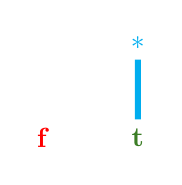
\begin{tikzpicture}[scale=0.4]
						\node (A) at (0,0) {\textcolor{red}{\textbf{f}}};
						\node (B) at (3,0) {\textcolor{OliveGreen}{\textbf{t}}};
						\node (C) at (3,3) {\textcolor{cyan}{$*$}};
						\draw[cyan, line width=.03in] (B) -- (C);
						\end{tikzpicture} \\
						\begin{tikzpicture}[scale=0.4]
							\node (A) at (0,0) {\textcolor{YellowOrange}{$\bigcdot$}};
						\end{tikzpicture}  && 
					
\begin{tikzpicture}[scale=0.35]
							\node (E) at (-6,0) {\textcolor{red}{$\bigcdot$}};			
			
							\node (A) at (0,0) {\textcolor{OliveGreen}{$\bigcdot$}};
							\node (A') at (0.5,-0.5) {\textcolor{YellowOrange}{$\bullet$}};
							\node (B) at (-3,3) {\textcolor{cyan}{$\bigcdot$}};
							\node (C) at (0,3) {\textcolor{cyan}{$\bigcdot$}};
							\node (D) at (3,3) {\textcolor{cyan}{$\bigcdot$}};
							\draw[cyan, line width=.03in] (A) -- (B);
							\draw[cyan, line width=.03in] (A) -- (C);
							\draw[cyan, line width=.03in] (A) -- (D);
							
							\node (A') at (9,0) {\textcolor{red}{$\bigcdot$}};
							\node (B') at (6,3) {\textcolor{red}{$\bigcdot$}};
							\node (C') at (9,3) {\textcolor{red}{$\bigcdot$}};
							\node (D') at (12,3) {\textcolor{red}{$\bigcdot$}};
							\draw[red, line width=.03in] (A') -- (B');
							\draw[red, line width=.03in] (A') -- (C');
							\draw[red, line width=.03in] (A') -- (D');
						\end{tikzpicture} \\
					& {} \\
						\begin{tikzpicture}[scale=0.4]
							\node (A) at (0,0) {\textcolor{OliveGreen}{$\bigcdot$}};
								\node (a) at (0.5,-0.5) {\textcolor{YellowOrange}{$\bullet$}};
						\end{tikzpicture} && 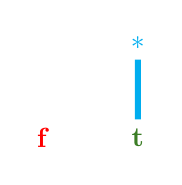
\begin{tikzpicture}[scale=0.4]
						\node (A) at (0,0) {\textcolor{red}{\textbf{f}}};
						\node (B) at (3,0) {\textcolor{OliveGreen}{\textbf{t}}};
						\node (C) at (3,3) {\textcolor{cyan}{$*$}};
						\draw[cyan, line width=.03in] (B) -- (C);
						\end{tikzpicture} 
					\arrow["{\ulcorner true_{\textbf{1}_\bot} \urcorner}", from=2-1, to=2-3]
					\arrow["{!_1}"', dashed, from=2-1, to=4-1]
					\arrow["true"', from=4-1, to=4-3]
					\arrow["{\forall_{\textbf{1}_\bot}}", from=2-3, to=4-3]
					\arrow["{true_{\textbf{1}_\bot} \circ \;\pi_{\textbf{1}_\bot} }"', from=1-1, to=1-3]
					\arrow[draw=none, from=2-1, to=3-2]
					\arrow[ from=2-1, to=3-2, phantom, "\scalebox{1.5}{$\lrcorner$}" , very near start, color=black]
				\end{tikzcd}
				\caption{ Pullback diagram for $\forall_{\textbf{1}_\bot}$ which is displayed with the usual coloring. Also we indicate the image of \textbf{1} with an orange bullet. }
		\end{figure}
\end{definition}

\newpage
 By definition $ \llbracket \forall x. \textbf{P}_t(x) \rrbracket = \forall_{\textbf{1}_\bot} \circ | \textbf{P}_t(x) |_1^1 $.
	\begin{figure}[h]
			\centering
			\begin{tikzcd}
					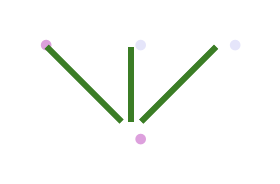
\begin{tikzpicture}[scale=0.4]
							\node (A) at (0,0) {\textcolor{OliveGreen}{$\bigcdot$}};
							\node (a) at (0.3,-0.3) {\textcolor{Plum}{$\bullet$}};
							\node (B) at (-3,3) {\textcolor{OliveGreen}{$\bigcdot$}};
							\node (b) at (-2.7,2.7) {\textcolor{Plum}{$\bullet$}};
							\node (C) at (0,3) {\textcolor{OliveGreen}{$\bigcdot$}};
							\node (c) at (0.3,2.7) {\textcolor{Lavender}{$\bullet$}};
							\node (D) at (3,3) {\textcolor{OliveGreen}{$\bigcdot$}};
							\node (d) at (3.3,2.7) {\textcolor{Lavender}{$\bullet$}};
							\draw[OliveGreen, line width=.03in] (A) -- (B);
							\draw[OliveGreen, line width=.03in] (A) -- (C);
							\draw[OliveGreen, line width=.03in] (A) -- (D);
						\end{tikzpicture} & 
\begin{tikzpicture}[scale=0.4]
							\node (A) at (0,0) {\textcolor{Plum}{$\bullet$}};
							\node (B) at (0,3) {\textcolor{Lavender}{$\bullet$}};
							\draw[Lavender, line width=.03in] (A) -- (B);
						\end{tikzpicture} & 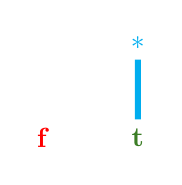
\begin{tikzpicture}[scale=0.4]
						\node (A) at (0,0) {\textcolor{red}{\textbf{f}}};
						\node (B) at (3,0) {\textcolor{OliveGreen}{\textbf{t}}};
						\node (C) at (3,3) {\textcolor{cyan}{$*$}};
						\draw[cyan, line width=.03in] (B) -- (C);
						\end{tikzpicture}  \\
					
\begin{tikzpicture}[scale=0.4]
							\node (A) at (0,0) {\textcolor{OliveGreen}{$\bigcdot$}};
							\node (a) at (0.5,-0.5) {\textcolor{YellowOrange}{$\bullet$}};
							\node (B) at (0,3) {\textcolor{OliveGreen}{$\bigcdot$}};
							\node (b) at (0.5,2.5) {\textcolor{yellow}{$\bullet$}};
							\draw[OliveGreen, line width=.03in] (A) -- (B);
						\end{tikzpicture}  && 
\begin{tikzpicture}[scale=0.35]
						\node (E) at (-6,0) {\textcolor{red}{$\bigcdot$}};			
						
						\node (A) at (0,0) {\textcolor{OliveGreen}{$\bigcdot$}};
						\node (a0) at (0.7,-0.7) {\textcolor{YellowOrange}{$\bullet$}};
						\node (a1) at (0.7,-0.2) {\textcolor{yellow}{$\bullet$}};
						\node (B) at (-3,3) {\textcolor{cyan}{$\bigcdot$}};
						\node (C) at (0,3) {\textcolor{cyan}{$\bigcdot$}};
						\node (D) at (3,3) {\textcolor{cyan}{$\bigcdot$}};
						\draw[cyan, line width=.03in] (A) -- (B);
						\draw[cyan, line width=.03in] (A) -- (C);
						\draw[cyan, line width=.03in] (A) -- (D);
						
						\node (A') at (9,0) {\textcolor{red}{$\bigcdot$}};
						\node (B') at (6,3) {\textcolor{red}{$\bigcdot$}};
						\node (C') at (9,3) {\textcolor{red}{$\bigcdot$}};
						\node (D') at (12,3) {\textcolor{red}{$\bigcdot$}};
						\draw[red, line width=.03in] (A') -- (B');
						\draw[red, line width=.03in] (A') -- (C');
						\draw[red, line width=.03in] (A') -- (D');
						\end{tikzpicture} \\
					\\
					&& 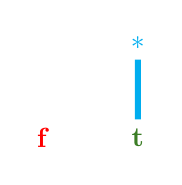
\begin{tikzpicture}[scale=0.4]
							\node (A) at (0,0) {\textcolor{red}{\textbf{f}}};
							\node (B) at (3,0) {\textcolor{OliveGreen}{\textbf{t}}};
							\node (C) at (3,3) {\textcolor{cyan}{$*$}};
							\draw[cyan, line width=.03in] (B) -- (C);
						\end{tikzpicture}
					\arrow["{| \textbf{P}_t(x) |_1^1}", from=2-1, to=2-3]
					\arrow["{\forall_{\textbf{1}_\bot}}", from=2-3, to=4-3]
					\arrow["{\llbracket \forall x.\textbf{P}_t(x) \rrbracket}"', from=2-1, to=4-3]
					\arrow["{pr_2^2}", from=1-1, to=1-2]
					\arrow["{\llbracket \textbf{P}_t(x) \rrbracket}", from=1-2, to=1-3]
				\end{tikzcd}
			\caption{  $ \llbracket \forall x. \textbf{P}_t(x) \rrbracket = true_{\textbf{1}_\bot} = \llbracket \textbf{P}_t(x) \rrbracket$. }
		\end{figure}
	
	In a similar fashion we find that $\llbracket \forall x. \textbf{P}_f(x) \rrbracket = \llbracket \textbf{P}_f(x) \rrbracket$.
	\newpage
	What happens with $\llbracket \forall x. \textbf{P}_*(x) \rrbracket$ ?
	\newline
	\newline
	 $ \llbracket \forall x. \textbf{P}_*(x) \rrbracket = \forall_{\textbf{1}_\bot} \circ | \textbf{P}_*(x) |_1^1 $
	\begin{figure}[h]
			\centering
			\begin{tikzcd}
					
\begin{tikzpicture}[scale=0.4]
							\node (A) at (0,0) {\textcolor{OliveGreen}{$\bigcdot$}};
							\node (a) at (0.3,-0.3) {\textcolor{Plum}{$\bullet$}};
							\node (B) at (-3,3) {\textcolor{OliveGreen}{$\bigcdot$}};
							\node (b) at (-2.7,2.7) {\textcolor{Plum}{$\bullet$}};
							\node (C) at (0,3) {\textcolor{cyan}{$\bigcdot$}};
							\node (c) at (0.3,2.7) {\textcolor{Lavender}{$\bullet$}};
							\node (D) at (3,3) {\textcolor{cyan}{$\bigcdot$}};
							\node (d) at (3.3,2.7) {\textcolor{Lavender}{$\bullet$}};
							\draw[OliveGreen, line width=.03in] (A) -- (B);
							\draw[cyan, line width=.03in] (A) -- (C);
							\draw[cyan, line width=.03in] (A) -- (D);
						\end{tikzpicture} & 
\begin{tikzpicture}[scale=0.4]
							\node (A) at (0,0) {\textcolor{Plum}{$\bullet$}};
							\node (B) at (0,3) {\textcolor{Lavender}{$\bullet$}};
							\draw[Lavender, line width=.03in] (A) -- (B);
						\end{tikzpicture} & 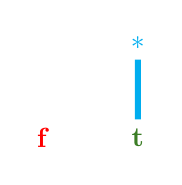
\begin{tikzpicture}[scale=0.4]
							\node (A) at (0,0) {\textcolor{red}{\textbf{f}}};
							\node (B) at (3,0) {\textcolor{OliveGreen}{\textbf{t}}};
							\node (C) at (3,3) {\textcolor{cyan}{$*$}};
							\draw[cyan, line width=.03in] (B) -- (C);
						\end{tikzpicture}  \\
					
\begin{tikzpicture}[scale=0.4]
							\node (A) at (0,0) {\textcolor{red}{$\bigcdot$}};
							\node (a) at (0.5,-0.5) {\textcolor{YellowOrange}{$\bullet$}};
							\node (B) at (0,3) {\textcolor{red}{$\bigcdot$}};
							\node (b) at (0.5,2.5) {\textcolor{yellow}{$\bullet$}};
							\draw[red, line width=.03in] (A) -- (B);
						\end{tikzpicture}  && 
\begin{tikzpicture}[scale=0.35]
							\node (E) at (-6,0) {\textcolor{red}{$\bigcdot$}};			
							
							\node (A) at (0,0) {\textcolor{OliveGreen}{$\bigcdot$}};
							\node (B) at (-3,3) {\textcolor{cyan}{$\bigcdot$}};
							\node (C) at (0,3) {\textcolor{cyan}{$\bigcdot$}};
							\node (D) at (3,3) {\textcolor{cyan}{$\bigcdot$}};
							\draw[cyan, line width=.03in] (A) -- (B);
							\draw[cyan, line width=.03in] (A) -- (C);
							\draw[cyan, line width=.03in] (A) -- (D);
							
							\node (A') at (9,0) {\textcolor{red}{$\bigcdot$}};
							\node (a0') at (9.7,-0.7) {\textcolor{YellowOrange}{$\bullet$}};
							\node (a1') at (9.7,-0.2) {\textcolor{yellow}{$\bullet$}};
							\node (B') at (6,3) {\textcolor{red}{$\bigcdot$}};
							\node (C') at (9,3) {\textcolor{red}{$\bigcdot$}};
							\node (D') at (12,3) {\textcolor{red}{$\bigcdot$}};
							\draw[red, line width=.03in] (A') -- (B');
							\draw[red, line width=.03in] (A') -- (C');
							\draw[red, line width=.03in] (A') -- (D');
						\end{tikzpicture} \\
					\\
					&& 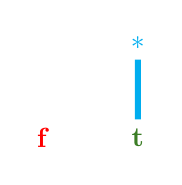
\begin{tikzpicture}[scale=0.4]
							\node (A) at (0,0) {\textcolor{red}{\textbf{f}}};
							\node (B) at (3,0) {\textcolor{OliveGreen}{\textbf{t}}};
							\node (C) at (3,3) {\textcolor{cyan}{$*$}};
							\draw[cyan, line width=.03in] (B) -- (C);
						\end{tikzpicture}
					\arrow["{| \textbf{P}_*(x) |_1^1}", from=2-1, to=2-3]
					\arrow["{\forall_{\textbf{1}_\bot}}", from=2-3, to=4-3]
					\arrow["{\llbracket \forall x.\textbf{P}_*(x) \rrbracket}"', from=2-1, to=4-3]
					\arrow["{pr_2^2}", from=1-1, to=1-2]
					\arrow["{\llbracket \textbf{P}_*(x) \rrbracket}", from=1-2, to=1-3]
				\end{tikzcd}
			\caption{	$ \llbracket \forall x. \textbf{P}_*(x) \rrbracket = \llbracket \textbf{P}_f(x) \rrbracket $. }
		\end{figure}
	
	
	
	\newpage
	\subsection{Interpreting $\exists$.}
	
	In order to obtain $ \exists_{\textbf{1}_\bot} $ one needs to examine the evaluation arrow $eval_{\textbf{1}_\bot} : \Omega^{\textbf{1}_\bot} \times \textbf{1}_\bot \rightarrow \textbf{1}_\bot$:
	
	\begin{figure}[h]
			\begin{tikzcd}
					
\begin{tikzpicture}[scale=0.3]
							\node (I) at (-28,-4) {\textcolor{red}{$\bigcdot$}};
							\node (J) at (-28,3) {\textcolor{red}{$\bigcdot$}};
							\draw[red, line width=.03in] (I) -- (J);
							
							\node (H) at (-22,3) {\textcolor{cyan}{$\bigcdot$}};
							\node (G) at (-19,3) {\textcolor{OliveGreen}{$\bigcdot$}};
							\node (F) at (-16,3) {\textcolor{cyan}{$\bigcdot$}};
							\node (A) at (-10,-4) {\textcolor{OliveGreen}{$\bigcdot$}};
							\node (B) at (-11,3) {\textcolor{OliveGreen}{$\bigcdot$}};
							\node (C) at (-8,3) {\textcolor{cyan}{$\bigcdot$}};
							\node (D) at (-5,3) {\textcolor{cyan}{$\bigcdot$}};
							\node (E) at (0,3) {\textcolor{OliveGreen}{$\bigcdot$}};
							\draw[OliveGreen, line width=.03in] (A) -- (B);
							\draw[cyan, line width=.03in] (A) -- (C);
							\draw[cyan, line width=.03in] (A) -- (D);
							\draw[OliveGreen, line width=.03in] (A) -- (E);
							\draw[cyan, line width=.03in] (A) -- (F);
							\draw[OliveGreen, line width=.03in] (A) -- (G);
							\draw[cyan, line width=.03in] (A) -- (H);
							
							\node (H') at (4,3) {\textcolor{OliveGreen}{$\bigcdot$}};
							\node (G') at (7,3) {\textcolor{cyan}{$\bigcdot$}};
							\node (F') at (10,3) {\textcolor{cyan}{$\bigcdot$}};
							\node (A') at (16,-4) {\textcolor{OliveGreen}{$\bigcdot$}};
							\node (B') at (15,3) {\textcolor{OliveGreen}{$\bigcdot$}};
							\node (C') at (18,3) {\textcolor{OliveGreen}{$\bigcdot$}};
							\node (D') at (21,3) {\textcolor{cyan}{$\bigcdot$}};
							\node (E') at (26,3) {\textcolor{cyan}{$\bullet$}};
							\draw[OliveGreen, line width=.03in] (A') -- (H');
							\draw[cyan, line width=.03in] (A') -- (G');
							\draw[cyan, line width=.03in] (A') -- (F');
							\draw[OliveGreen, line width=.03in] (A') -- (B');
							\draw[OliveGreen, line width=.03in] (A') -- (C');
							\draw[cyan, line width=.03in] (A') -- (D');
							\draw[cyan, line width=.03in] (A') -- (E');
							
							
						\end{tikzpicture} \\
					\\
				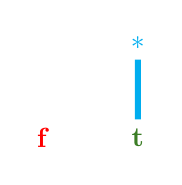
\begin{tikzpicture}[scale=0.4]
						\node (A) at (0,0) {\textcolor{red}{\textbf{f}}};
						\node (B) at (3,0) {\textcolor{OliveGreen}{\textbf{t}}};
						\node (C) at (3,3) {\textcolor{cyan}{$*$}};
						\draw[cyan, line width=.03in] (B) -- (C);
					\end{tikzpicture}
					\arrow["eval"', from=1-1, to=3-1]
				\end{tikzcd}
			\caption{$eval_{\textbf{1}_\bot} : \Omega^{\textbf{1}_\bot} \times \textbf{1}_\bot \rightarrow \textbf{1}_\bot$ with the usual coloring notation.}
		\end{figure}
	
	
	
	 \begin{definition}[$\exists_{\textbf{1}_\bot}$]
			$\exists_{\textbf{1}_\bot}$ is the characteristic of the image arrow of  $p_{\textbf{1}_\bot} \circ \in_{\textbf{1}_\bot}$ with $p_{\textbf{1}_\bot}$ being the projection on $\Omega^{\textbf{1}_\bot}$ and $\in_{\textbf{1}_\bot}$  the sub-object of $\Omega^{\textbf{1}_\bot} \times {\textbf{1}_\bot}$ whose character is the evaluation arrow $eval_{\textbf{1}_\bot}: \Omega^{\textbf{1}_\bot} \times {\textbf{1}_\bot} \rightarrow {\textbf{1}_\bot}$.
			
			\begin{figure}[h]
					\centering
					\begin{tikzcd}
										
\begin{tikzpicture}[scale=0.15]
							
									
									\node (G) at (-19,3) {\textcolor{Plum}{$\bullet$}};
									\node (A) at (-10,-6) {\textcolor{Plum}{$\bullet$}};
									\node (B) at (-11,3) {\textcolor{Plum}{$\bullet$}};
									\node (E) at (0,3) {\textcolor{Plum}{$\bullet$}};
									\draw[Plum, line width=.03in] (A) -- (B);
									\draw[Plum, line width=.03in] (A) -- (E);
									\draw[Plum, line width=.03in] (A) -- (G);
								
									
									\node (H') at (4,3) {\textcolor{Plum}{$\bullet$}};
									\node (A') at (16,-6) {\textcolor{Plum}{$\bullet$}};
									\node (B') at (15,3) {\textcolor{Plum}{$\bullet$}};
									\node (C') at (18,3) {\textcolor{Plum}{$\bullet$}};
									\draw[Plum, line width=.03in] (A') -- (H');
									\draw[Plum, line width=.03in] (A') -- (B');
									\draw[Plum, line width=.03in] (A') -- (C');
									
									
								\end{tikzpicture} && 			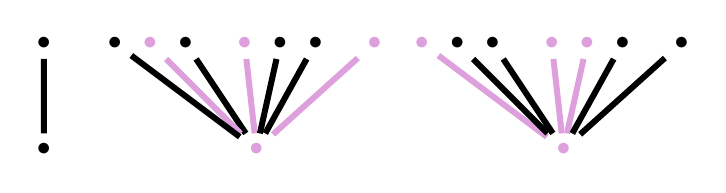
\begin{tikzpicture}[scale=0.15]
									\node (I) at (-28,-6) {\textcolor{black}{$\bullet$}};
									\node (J) at (-28,3) {\textcolor{black}{$\bullet$}};
									\draw[ line width=.03in] (I) -- (J);
									
									\node (H) at (-22,3) {\textcolor{black}{$\bullet$}};
									\node (G) at (-19,3) {\textcolor{Plum}{$\bullet$}};
									\node (F) at (-16,3) {\textcolor{black}{$\bullet$}};
									\node (A) at (-10,-6) {\textcolor{Plum}{$\bullet$}};
									\node (B) at (-11,3) {\textcolor{Plum}{$\bullet$}};
									\node (C) at (-8,3) {\textcolor{black}{$\bullet$}};
									\node (D) at (-5,3) {\textcolor{black}{$\bullet$}};
									\node (E) at (0,3) {\textcolor{Plum}{$\bullet$}};
									\draw[Plum, line width=.03in] (A) -- (B);
									\draw[black, line width=.03in] (A) -- (C);
									\draw[black, line width=.03in] (A) -- (D);
									\draw[Plum, line width=.03in] (A) -- (E);
									\draw[black, line width=.03in] (A) -- (F);
									\draw[Plum, line width=.03in] (A) -- (G);
									\draw[black, line width=.03in] (A) -- (H);
									
									\node (H') at (4,3) {\textcolor{Plum}{$\bullet$}};
									\node (G') at (7,3) {\textcolor{black}{$\bullet$}};
									\node (F') at (10,3) {\textcolor{black}{$\bullet$}};
									\node (A') at (16,-6) {\textcolor{Plum}{$\bullet$}};
									\node (B') at (15,3) {\textcolor{Plum}{$\bullet$}};
									\node (C') at (18,3) {\textcolor{Plum}{$\bullet$}};
									\node (D') at (21,3) {\textcolor{black}{$\bullet$}};
									\node (E') at (26,3) {\textcolor{black}{$\bullet$}};
									\draw[Plum, line width=.03in] (A') -- (H');
									\draw[black, line width=.03in] (A') -- (G');
									\draw[black, line width=.03in] (A') -- (F');
									\draw[Plum, line width=.03in] (A') -- (B');
									\draw[Plum, line width=.03in] (A') -- (C');
									\draw[black, line width=.03in] (A') -- (D');
									\draw[black, line width=.03in] (A') -- (E');
									
									
								\end{tikzpicture} \\
							\\
							
\begin{tikzpicture}[scale=0.35]	
									\node (A) at (0,0) {\textcolor{black}{$\bigcdot$}};
									\node (B) at (-3,3) {\textcolor{black}{$\bigcdot$}};
									\node (C) at (0,3) {\textcolor{black}{$\bigcdot$}};
									\draw[black, line width=.03in] (A) -- (B);
									\draw[black, line width=.03in] (A) -- (C);
									
									\node (A') at (9,0) {\textcolor{black}{$\bigcdot$}};
									\node (B') at (6,3) {\textcolor{black}{$\bigcdot$}};
									\node (C') at (9,3) {\textcolor{black}{$\bigcdot$}};
									\draw[black, line width=.03in] (A') -- (B');
									\draw[black, line width=.03in] (A') -- (C');
								\end{tikzpicture} && 
							
\begin{tikzpicture}[scale=0.35]
									\node (E) at (-6,0) {\textcolor{red}{$\bigcdot$}};			
									
									\node (A) at (0,0) {\textcolor{OliveGreen}{$\bigcdot$}};
									\node (B) at (-3,3) {\textcolor{OliveGreen}{$\bigcdot$}};
									\node (C) at (0,3) {\textcolor{OliveGreen}{$\bigcdot$}};
									\node (D) at (3,3) {\textcolor{cyan}{$\bigcdot$}};
									\draw[OliveGreen, line width=.03in] (A) -- (B);
									\draw[OliveGreen, line width=.03in] (A) -- (C);
									\draw[cyan, line width=.03in] (A) -- (D);
									
									\node (A') at (9,0) {\textcolor{OliveGreen}{$\bigcdot$}};
									\node (B') at (6,3) {\textcolor{OliveGreen}{$\bigcdot$}};
									\node (C') at (9,3) {\textcolor{OliveGreen}{$\bigcdot$}};
									\node (D') at (12,3) {\textcolor{cyan}{$\bigcdot$}};
									\draw[OliveGreen, line width=.03in] (A') -- (B');
									\draw[OliveGreen, line width=.03in] (A') -- (C');
									\draw[cyan, line width=.03in] (A') -- (D');
								\end{tikzpicture} \\
							& {} \\
						\begin{tikzpicture}[scale=0.4]
								\node (A) at (0,0) {\textcolor{OliveGreen}{$\bigcdot$}};
							\end{tikzpicture} && 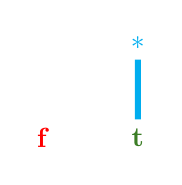
\begin{tikzpicture}[scale=0.4]
									\node (A) at (0,0) {\textcolor{red}{\textbf{f}}};
									\node (B) at (3,0) {\textcolor{OliveGreen}{\textbf{t}}};
									\node (C) at (3,3) {\textcolor{cyan}{$*$}};
									\draw[cyan, line width=.03in] (B) -- (C);
								\end{tikzpicture}
							\arrow["{im(p_{\textbf{1}_\bot} \circ \in_{\textbf{1}_\bot}) }", tail, from=3-1, to=3-3]
							\arrow["{!_1}"', dashed, from=3-1, to=5-1]
							\arrow["true"', from=5-1, to=5-3]
							\arrow["{\exists_{\textbf{1}_\bot}}", from=3-3, to=5-3]
							\arrow[draw=none, from=3-1, to=4-2]
							\arrow[ from=3-1, to=4-2, phantom, "\scalebox{1.5}{$\lrcorner$}" , very near start, color=black]
							\arrow["{\in_{\textbf{1}_\bot}}", tail, from=1-1, to=1-3]
							\arrow["{p_{\textbf{1}_\bot}}", from=1-3, to=3-3]
							\arrow[two heads, from=1-1, to=3-1]
						\end{tikzcd}
					\caption{the bottom square is a pull-back while the top square is an epi-mono factorization for $p_{\textbf{1}_\bot} \circ \in_{\textbf{1}_\bot}$. }
				\end{figure}
		\end{definition}
	\newpage
	 By definition $ \llbracket \exists x. \textbf{P}_t(x) \rrbracket = \exists_{\textbf{1}_\bot} \circ | \textbf{P}_t(x) |_1^1 $ and we find that:
	\newline
	$ \llbracket \exists x. \textbf{P}_t(x) \rrbracket = true_{\textbf{1}_\bot} = \llbracket \textbf{P}_t(x) \rrbracket$.  
	\begin{figure}[h]
			\centering
			\begin{tikzcd}
					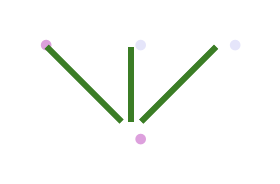
\begin{tikzpicture}[scale=0.4]
							\node (A) at (0,0) {\textcolor{OliveGreen}{$\bigcdot$}};
							\node (a) at (0.3,-0.3) {\textcolor{Plum}{$\bullet$}};
							\node (B) at (-3,3) {\textcolor{OliveGreen}{$\bigcdot$}};
							\node (b) at (-2.7,2.7) {\textcolor{Plum}{$\bullet$}};
							\node (C) at (0,3) {\textcolor{OliveGreen}{$\bigcdot$}};
							\node (c) at (0.3,2.7) {\textcolor{Lavender}{$\bullet$}};
							\node (D) at (3,3) {\textcolor{OliveGreen}{$\bigcdot$}};
							\node (d) at (3.3,2.7) {\textcolor{Lavender}{$\bullet$}};
							\draw[OliveGreen, line width=.03in] (A) -- (B);
							\draw[OliveGreen, line width=.03in] (A) -- (C);
							\draw[OliveGreen, line width=.03in] (A) -- (D);
						\end{tikzpicture} & 
\begin{tikzpicture}[scale=0.4]
							\node (A) at (0,0) {\textcolor{Plum}{$\bullet$}};
							\node (B) at (0,3) {\textcolor{Lavender}{$\bullet$}};
							\draw[Lavender, line width=.03in] (A) -- (B);
						\end{tikzpicture} & 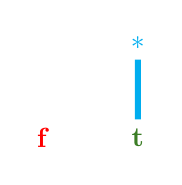
\begin{tikzpicture}[scale=0.4]
							\node (A) at (0,0) {\textcolor{red}{\textbf{f}}};
							\node (B) at (3,0) {\textcolor{OliveGreen}{\textbf{t}}};
							\node (C) at (3,3) {\textcolor{cyan}{$*$}};
							\draw[cyan, line width=.03in] (B) -- (C);
						\end{tikzpicture}  \\
					
\begin{tikzpicture}[scale=0.4]
							\node (A) at (0,0) {\textcolor{OliveGreen}{$\bigcdot$}};
							\node (a) at (0.5,-0.5) {\textcolor{YellowOrange}{$\bullet$}};
							\node (B) at (0,3) {\textcolor{OliveGreen}{$\bigcdot$}};
							\node (b) at (0.5,2.5) {\textcolor{yellow}{$\bullet$}};
							\draw[OliveGreen, line width=.03in] (A) -- (B);
						\end{tikzpicture}  && 
\begin{tikzpicture}[scale=0.35]
						\node (E) at (-6,0) {\textcolor{red}{$\bigcdot$}};			
						
						\node (A) at (0,0) {\textcolor{OliveGreen}{$\bigcdot$}};
						\node (a0') at (0.7,-0.7) {\textcolor{YellowOrange}{$\bullet$}};
						\node (a1') at (0.7,-0.2) {\textcolor{yellow}{$\bullet$}};
						\node (B) at (-3,3) {\textcolor{OliveGreen}{$\bigcdot$}};
						\node (C) at (0,3) {\textcolor{OliveGreen}{$\bigcdot$}};
						\node (D) at (3,3) {\textcolor{cyan}{$\bigcdot$}};
						\draw[OliveGreen, line width=.03in] (A) -- (B);
						\draw[OliveGreen, line width=.03in] (A) -- (C);
						\draw[cyan, line width=.03in] (A) -- (D);
						
						\node (A') at (9,0) {\textcolor{OliveGreen}{$\bigcdot$}};
						\node (B') at (6,3) {\textcolor{OliveGreen}{$\bigcdot$}};
						\node (C') at (9,3) {\textcolor{OliveGreen}{$\bigcdot$}};
						\node (D') at (12,3) {\textcolor{cyan}{$\bigcdot$}};
						\draw[OliveGreen, line width=.03in] (A') -- (B');
						\draw[OliveGreen, line width=.03in] (A') -- (C');
						\draw[cyan, line width=.03in] (A') -- (D');
						\end{tikzpicture} \\
					\\
					&& 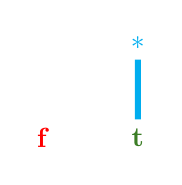
\begin{tikzpicture}[scale=0.4]
							\node (A) at (0,0) {\textcolor{red}{\textbf{f}}};
							\node (B) at (3,0) {\textcolor{OliveGreen}{\textbf{t}}};
							\node (C) at (3,3) {\textcolor{cyan}{$*$}};
							\draw[cyan, line width=.03in] (B) -- (C);
						\end{tikzpicture}
					\arrow["{| \textbf{P}_t(x) |_1^1}", from=2-1, to=2-3]
					\arrow["{\exists_{\textbf{1}_\bot}}", from=2-3, to=4-3]
					\arrow["{\llbracket \exists x.\textbf{P}_t(x) \rrbracket}"', from=2-1, to=4-3]
					\arrow["{pr_2^2}", from=1-1, to=1-2]
					\arrow["{\llbracket \textbf{P}_t(x) \rrbracket}", from=1-2, to=1-3]
				\end{tikzcd}
			\caption{ $\llbracket \exists x. \textbf{P}_f(x) \rrbracket = \llbracket \textbf{P}_f(x) \rrbracket$.}
		\end{figure}
	
		In a similar way as before we conclude: \newline

		 $\llbracket \exists x. \textbf{P}_*(x) \rrbracket = \llbracket \textbf{P}_t(x) \rrbracket$.
		 
		 \newpage
		 \subsection{Expanding the Context.}
		 
		 
		 \begin{ex} (m=2)
			 	\begin{gather*}
				 		\textfrak{X}= \langle \textbf{1}_\bot, \{\textfrak{p}_t, \textfrak{p}_f, \textfrak{p}_*\}, \textfrak{f}_c \rangle. \\ \\
				 		\llbracket x_1 \rrbracket = {pr_1} : (\textbf{1}_\bot \times \textbf{1}_\bot) \rightarrow \textbf{1}_\bot. \\
				 		\llbracket x_2 \rrbracket = {pr_2} : (\textbf{1}_\bot \times \textbf{1}_\bot) \rightarrow \textbf{1}_\bot. \\
				 		\llbracket \textbf{c} \rrbracket = \textfrak{f}_c \circ !_{\textbf{1}_\bot \times \textbf{1}_\bot} : (\textbf{1}_\bot \times \textbf{1}_\bot) \rightarrow \textbf{1}_\bot.  \\
				 		\llbracket \textbf{P}_t (x_1) \rrbracket = \textfrak{P}_t \circ \llbracket x_1 \rrbracket = \textfrak{P}_t \circ pr_1 : (\textbf{1}_\bot \times \textbf{1}_\bot)  \rightarrow \Omega.\\
				 		...
				 		\end{gather*}
			 \end{ex}
		 
		 \begin{equation*}
			 	(\textbf{1}_\bot)^3 = (\textbf{1}_\bot)^2 \times (\textbf{1}_\bot) = ( 3\cdot(\textbf{1}_\bot) + 3\cdot(\textbf{1}) + (\textbf{1}_\bot)^2 )_\bot \cong_{\mathbb{FF_2}} (7\cdot\textbf{1})_\bot 
			 \end{equation*}

		 \begin{figure}[h]
			 	\centering
			 	\begin{tikzcd}
				 		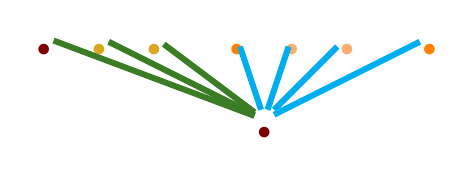
\begin{tikzpicture}[scale=0.35]
					 			\node (H) at (-8,3) {\textcolor{OliveGreen}{$\bigcdot$}};
					 			\node (h) at (-8,2.5) {\textcolor{Maroon}{$\bullet$}};
					 			\node (G) at (-6,3) {\textcolor{OliveGreen}{$\bigcdot$}};
					 			\node (g) at (-6,2.5) {\textcolor{Goldenrod}{$\bullet$}};
					 			\node (F) at (-4,3) {\textcolor{OliveGreen}{$\bigcdot$}};
					 			\node (f) at (-4,2.5) {\textcolor{Goldenrod}{$\bullet$}};
					 		\node (A) at (0,0) {\textcolor{OliveGreen}{$\bigcdot$}};
					 		\node (a) at (0,-0.5) {\textcolor{Maroon}{$\bullet$}};
					 			\node (B) at (-1,3) {\textcolor{cyan}{$\bigcdot$}};
					 			\node (b) at (-1,2.5) {\textcolor{orange}{$\bullet$}};
					 			\node (C) at (1,3) {\textcolor{cyan}{$\bigcdot$}};
					 			\node (c) at (1,2.5) {\textcolor{Apricot}{$\bullet$}};
					 			\node (D) at (3,3) {\textcolor{cyan}{$\bigcdot$}};
					 			\node (d) at (3,2.5) {\textcolor{Apricot}{$\bullet$}};
					 			\node (E) at (6,3) {\textcolor{cyan}{$\bigcdot$}};
					 			\node (e) at (6,2.5) {\textcolor{orange}{$\bullet$}};
					 			\draw[cyan, line width=.03in] (A) -- (B);
					 			\draw[cyan, line width=.03in] (A) -- (C);
					 			\draw[cyan, line width=.03in] (A) -- (D);
					 			\draw[cyan, line width=.03in] (A) -- (E);
					 			\draw[OliveGreen, line width=.03in] (A) -- (F);
					 			\draw[OliveGreen, line width=.03in] (A) -- (G);
					 			\draw[OliveGreen, line width=.03in] (A) -- (H);
					 		\end{tikzpicture} & 	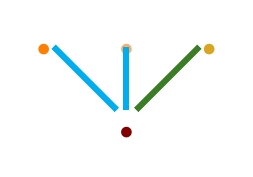
\begin{tikzpicture}[scale=0.35]
					 		\node (A) at (0,0) {\textcolor{OliveGreen}{$\bigcdot$}};
					 		\node (a) at (0,-0.5) {\textcolor{Maroon}{$\bullet$}};
					 		\node (B) at (-3,3) {\textcolor{cyan}{$\bigcdot$}};
					 		\node (b) at (-3,2.5) {\textcolor{orange}{$\bullet$}};
					 		\node (C) at (0,3) {\textcolor{cyan}{$\bigcdot$}};
					 		\node (c) at (0,2.5) {\textcolor{Apricot}{$\bullet$}};
					 		\node (D) at (3,3) {\textcolor{OliveGreen}{$\bigcdot$}};
					 		\node (d) at (3,2.5) {\textcolor{Goldenrod}{$\bullet$}};
					 		\draw[cyan, line width=.03in] (A) -- (B);
					 		\draw[cyan, line width=.03in] (A) -- (C);
					 		\draw[OliveGreen, line width=.03in] (A) -- (D);
					 		\end{tikzpicture} & 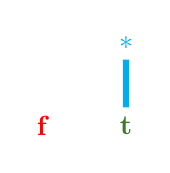
\begin{tikzpicture}[scale=0.35]
					 		\node (A) at (0,0) {\textcolor{red}{\textbf{f}}};
					 		\node (B) at (3,0) {\textcolor{OliveGreen}{\textbf{t}}};
					 		\node (C) at (3,3) {\textcolor{cyan}{$*$}};
					 		\draw[cyan, line width=.03in] (B) -- (C);
					 		\end{tikzpicture} \\
				 		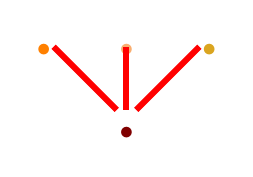
\begin{tikzpicture}[scale=0.35]
					 			\node (A) at (0,0) {\textcolor{red}{$\bigcdot$}};
					 			\node (a) at (0,-0.5) {\textcolor{Maroon}{$\bullet$}};
					 			\node (B) at (-3,3) {\textcolor{red}{$\bigcdot$}};
					 			\node (b) at (-3,2.5) {\textcolor{orange}{$\bullet$}};
					 			\node (C) at (0,3) {\textcolor{red}{$\bigcdot$}};
					 			\node (c) at (0,2.5) {\textcolor{Apricot}{$\bullet$}};
					 			\node (D) at (3,3) {\textcolor{red}{$\bigcdot$}};
					 			\node (d) at (3,2.5) {\textcolor{Goldenrod}{$\bullet$}};
					 			\draw[red, line width=.03in] (A) -- (B);
					 			\draw[red, line width=.03in] (A) -- (C);
					 			\draw[red, line width=.03in] (A) -- (D);
					 		\end{tikzpicture} & 
\begin{tikzpicture}[scale=0.35]
					 		\node (E) at (-6,0) {\textcolor{red}{$\bigcdot$}};			
					 		
					 		\node (A) at (0,0) {\textcolor{OliveGreen}{$\bigcdot$}};
					 		\node (B) at (-3,3) {\textcolor{cyan}{$\bigcdot$}};
					 		\node (C) at (0,3) {\textcolor{cyan}{$\bigcdot$}};
					 		\node (D) at (3,3) {\textcolor{cyan}{$\bigcdot$}};
					 		\draw[cyan, line width=.03in] (A) -- (B);
					 		\draw[cyan, line width=.03in] (A) -- (C);
					 		\draw[cyan, line width=.03in] (A) -- (D);
					 		
					 		\node (A') at (9,0) {\textcolor{red}{$\bigcdot$}};
					 		\node (a) at (9,-1) {\textcolor{Maroon}{$\bullet$}};
					 		\node (a') at (8.5,-0.5) {\textcolor{orange}{$\bullet$}};
					 		\node (a'') at (9,-0.5) {\textcolor{Apricot}{$\bullet$}};
					 		\node (a''') at (9.5,-0.5) {\textcolor{Goldenrod}{$\bullet$}};
					 		\node (B') at (6,3) {\textcolor{red}{$\bigcdot$}};
					 		\node (C') at (9,3) {\textcolor{red}{$\bigcdot$}};
					 		\node (D') at (12,3) {\textcolor{red}{$\bigcdot$}};
					 		\draw[red, line width=.03in] (A') -- (B');
					 		\draw[red, line width=.03in] (A') -- (C');
					 		\draw[red, line width=.03in] (A') -- (D');
					 		\end{tikzpicture}  \\
				 		& 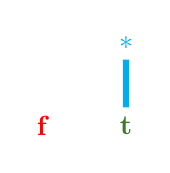
\begin{tikzpicture}[scale=0.35]
					 			\node (A) at (0,0) {\textcolor{red}{\textbf{f}}};
					 			\node (B) at (3,0) {\textcolor{OliveGreen}{\textbf{t}}};
					 			\node (C) at (3,3) {\textcolor{cyan}{$*$}};
					 			\draw[cyan, line width=.03in] (B) -- (C);
					 		\end{tikzpicture}
				 		\arrow["{pr^3_3 \times pr^3_2}"', from=1-1, to=1-2]
				 		\arrow["{\llbracket \textbf{P}_*(x_1) \rrbracket}"', from=1-2, to=1-3]
				 		\arrow["{| \textbf{P}_*(x_1) |_1^2}", from=2-1, to=2-2]
				 		\arrow["{\forall_{\textbf{1}_\bot}}", from=2-2, to=3-2]
				 		\arrow["{\llbracket \forall x_1.\textbf{P}_*(x_1) \rrbracket}"', from=2-1, to=3-2]
				 	\end{tikzcd}
			 	\caption{ 
				 		Again, we find:
				 		$ \llbracket \forall x_1. \textbf{P}_*(x_1) \rrbracket = \llbracket \textbf{P}_f(x_1) \rrbracket $.  }
			 \end{figure}
		 
		 	
		 		 \begin{figure}[h]
			 	\centering
			 	\begin{tikzcd}
				 		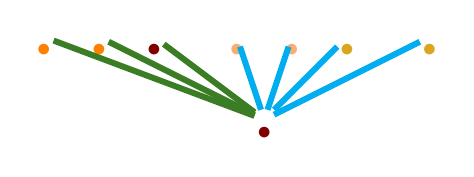
\begin{tikzpicture}[scale=0.35]
					 			\node (H) at (-8,3) {\textcolor{OliveGreen}{$\bigcdot$}};
					 			\node (h) at (-8,2.5) {\textcolor{orange}{$\bullet$}};
					 			\node (G) at (-6,3) {\textcolor{OliveGreen}{$\bigcdot$}};
					 			\node (g) at (-6,2.5) {\textcolor{orange}{$\bullet$}};
					 			\node (F) at (-4,3) {\textcolor{OliveGreen}{$\bigcdot$}};
					 			\node (f) at (-4,2.5) {\textcolor{Maroon}{$\bullet$}};
					 			\node (A) at (0,0) {\textcolor{OliveGreen}{$\bigcdot$}};
					 			\node (a) at (0,-0.5) {\textcolor{Maroon}{$\bullet$}};
					 			\node (B) at (-1,3) {\textcolor{cyan}{$\bigcdot$}};
					 			\node (b) at (-1,2.5) {\textcolor{Apricot}{$\bullet$}};
					 			\node (C) at (1,3) {\textcolor{cyan}{$\bigcdot$}};
					 			\node (c) at (1,2.5) {\textcolor{Apricot}{$\bullet$}};
					 			\node (D) at (3,3) {\textcolor{cyan}{$\bigcdot$}};
					 			\node (d) at (3,2.5) {\textcolor{Goldenrod}{$\bullet$}};
					 			\node (E) at (6,3) {\textcolor{cyan}{$\bigcdot$}};
					 			\node (e) at (6,2.5) {\textcolor{Goldenrod}{$\bullet$}};
					 			\draw[cyan, line width=.03in] (A) -- (B);
					 			\draw[cyan, line width=.03in] (A) -- (C);
					 			\draw[cyan, line width=.03in] (A) -- (D);
					 			\draw[cyan, line width=.03in] (A) -- (E);
					 			\draw[OliveGreen, line width=.03in] (A) -- (F);
					 			\draw[OliveGreen, line width=.03in] (A) -- (G);
					 			\draw[OliveGreen, line width=.03in] (A) -- (H);
					 		\end{tikzpicture} & 	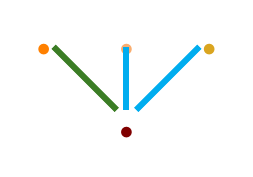
\begin{tikzpicture}[scale=0.35]
					 			\node (A) at (0,0) {\textcolor{OliveGreen}{$\bigcdot$}};
					 			\node (a) at (0,-0.5) {\textcolor{Maroon}{$\bullet$}};
					 			\node (B) at (-3,3) {\textcolor{OliveGreen}{$\bigcdot$}};
					 			\node (b) at (-3,2.5) {\textcolor{orange}{$\bullet$}};
					 			\node (C) at (0,3) {\textcolor{cyan}{$\bigcdot$}};
					 			\node (c) at (0,2.5) {\textcolor{Apricot}{$\bullet$}};
					 			\node (D) at (3,3) {\textcolor{cyan}{$\bigcdot$}};
					 			\node (d) at (3,2.5) {\textcolor{Goldenrod}{$\bullet$}};
					 			\draw[OliveGreen, line width=.03in] (A) -- (B);
					 			\draw[cyan, line width=.03in] (A) -- (C);
					 			\draw[cyan, line width=.03in] (A) -- (D);
					 		\end{tikzpicture} & 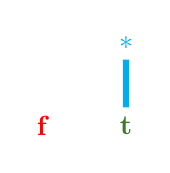
\begin{tikzpicture}[scale=0.35]
					 			\node (A) at (0,0) {\textcolor{red}{\textbf{f}}};
					 			\node (B) at (3,0) {\textcolor{OliveGreen}{\textbf{t}}};
					 			\node (C) at (3,3) {\textcolor{cyan}{$*$}};
					 			\draw[cyan, line width=.03in] (B) -- (C);
					 		\end{tikzpicture} \\
				 		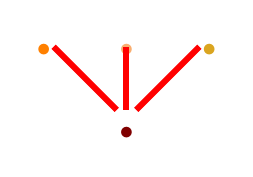
\begin{tikzpicture}[scale=0.35]
					 			\node (A) at (0,0) {\textcolor{red}{$\bigcdot$}};
					 			\node (a) at (0,-0.5) {\textcolor{Maroon}{$\bullet$}};
					 			\node (B) at (-3,3) {\textcolor{red}{$\bigcdot$}};
					 			\node (b) at (-3,2.5) {\textcolor{orange}{$\bullet$}};
					 			\node (C) at (0,3) {\textcolor{red}{$\bigcdot$}};
					 			\node (c) at (0,2.5) {\textcolor{Apricot}{$\bullet$}};
					 			\node (D) at (3,3) {\textcolor{red}{$\bigcdot$}};
					 			\node (d) at (3,2.5) {\textcolor{Goldenrod}{$\bullet$}};
					 			\draw[red, line width=.03in] (A) -- (B);
					 			\draw[red, line width=.03in] (A) -- (C);
					 			\draw[red, line width=.03in] (A) -- (D);
					 		\end{tikzpicture} & 
\begin{tikzpicture}[scale=0.35]
					 			\node (E) at (-6,0) {\textcolor{red}{$\bigcdot$}};			
					 			
					 			\node (A) at (0,0) {\textcolor{OliveGreen}{$\bigcdot$}};
					 			\node (B) at (-3,3) {\textcolor{cyan}{$\bigcdot$}};
					 			\node (C) at (0,3) {\textcolor{cyan}{$\bigcdot$}};
					 			\node (D) at (3,3) {\textcolor{cyan}{$\bigcdot$}};
					 			\draw[cyan, line width=.03in] (A) -- (B);
					 			\draw[cyan, line width=.03in] (A) -- (C);
					 			\draw[cyan, line width=.03in] (A) -- (D);
					 			
					 			\node (A') at (9,0) {\textcolor{red}{$\bigcdot$}};
					 			\node (a) at (9,-1) {\textcolor{Maroon}{$\bullet$}};
					 			\node (a') at (8.5,-0.5) {\textcolor{orange}{$\bullet$}};
					 			\node (a'') at (9,-0.5) {\textcolor{Apricot}{$\bullet$}};
					 			\node (a''') at (9.5,-0.5) {\textcolor{Goldenrod}{$\bullet$}};
					 			\node (B') at (6,3) {\textcolor{red}{$\bigcdot$}};
					 			\node (C') at (9,3) {\textcolor{red}{$\bigcdot$}};
					 			\node (D') at (12,3) {\textcolor{red}{$\bigcdot$}};
					 			\draw[red, line width=.03in] (A') -- (B');
					 			\draw[red, line width=.03in] (A') -- (C');
					 			\draw[red, line width=.03in] (A') -- (D');
					 		\end{tikzpicture}  \\
				 		& 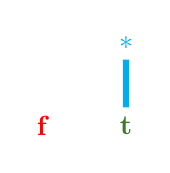
\begin{tikzpicture}[scale=0.35]
					 			\node (A) at (0,0) {\textcolor{red}{\textbf{f}}};
					 			\node (B) at (3,0) {\textcolor{OliveGreen}{\textbf{t}}};
					 			\node (C) at (3,3) {\textcolor{cyan}{$*$}};
					 			\draw[cyan, line width=.03in] (B) -- (C);
					 		\end{tikzpicture}
				 		\arrow["{pr^1_3 \times pr^3_3}"', from=1-1, to=1-2]
				 		\arrow["{\llbracket \textbf{P}_*(x_2) \rrbracket}"', from=1-2, to=1-3]
				 		\arrow["{| \textbf{P}_*(x_2) |_1^2}", from=2-1, to=2-2]
				 		\arrow["{\forall_{\textbf{1}_\bot}}", from=2-2, to=3-2]
				 		\arrow["{\llbracket \forall x_2.\textbf{P}_*(x_2) \rrbracket}"', from=2-1, to=3-2]
				 	\end{tikzcd}
			 	\caption{ Also:	$ \llbracket \forall x_2. \textbf{P}_*(x_2) \rrbracket = \llbracket \textbf{P}_f(x_2) \rrbracket $.}
			 \end{figure}	
		 
		
		 Moving on to existentials: 
		
\begin{figure}[h]
		 	\centering
		 	\begin{tikzcd}
			 		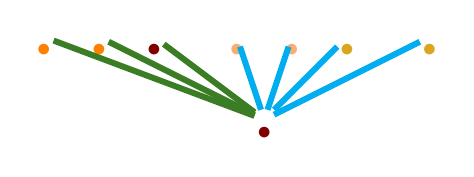
\begin{tikzpicture}[scale=0.35]
				 			\node (H) at (-8,3) {\textcolor{OliveGreen}{$\bigcdot$}};
				 			\node (h) at (-8,2.5) {\textcolor{orange}{$\bullet$}};
				 			\node (G) at (-6,3) {\textcolor{OliveGreen}{$\bigcdot$}};
				 			\node (g) at (-6,2.5) {\textcolor{orange}{$\bullet$}};
				 			\node (F) at (-4,3) {\textcolor{OliveGreen}{$\bigcdot$}};
				 			\node (f) at (-4,2.5) {\textcolor{Maroon}{$\bullet$}};
				 			\node (A) at (0,0) {\textcolor{OliveGreen}{$\bigcdot$}};
				 			\node (a) at (0,-0.5) {\textcolor{Maroon}{$\bullet$}};
				 			\node (B) at (-1,3) {\textcolor{cyan}{$\bigcdot$}};
				 			\node (b) at (-1,2.5) {\textcolor{Apricot}{$\bullet$}};
				 			\node (C) at (1,3) {\textcolor{cyan}{$\bigcdot$}};
				 			\node (c) at (1,2.5) {\textcolor{Apricot}{$\bullet$}};
				 			\node (D) at (3,3) {\textcolor{cyan}{$\bigcdot$}};
				 			\node (d) at (3,2.5) {\textcolor{Goldenrod}{$\bullet$}};
				 			\node (E) at (6,3) {\textcolor{cyan}{$\bigcdot$}};
				 			\node (e) at (6,2.5) {\textcolor{Goldenrod}{$\bullet$}};
				 			\draw[cyan, line width=.03in] (A) -- (B);
				 			\draw[cyan, line width=.03in] (A) -- (C);
				 			\draw[cyan, line width=.03in] (A) -- (D);
				 			\draw[cyan, line width=.03in] (A) -- (E);
				 			\draw[OliveGreen, line width=.03in] (A) -- (F);
				 			\draw[OliveGreen, line width=.03in] (A) -- (G);
				 			\draw[OliveGreen, line width=.03in] (A) -- (H);
				 		\end{tikzpicture} & 	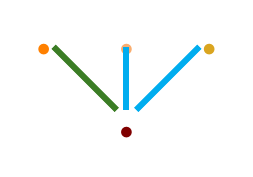
\begin{tikzpicture}[scale=0.35]
				 			\node (A) at (0,0) {\textcolor{OliveGreen}{$\bigcdot$}};
				 			\node (a) at (0,-0.5) {\textcolor{Maroon}{$\bullet$}};
				 			\node (B) at (-3,3) {\textcolor{OliveGreen}{$\bigcdot$}};
				 			\node (b) at (-3,2.5) {\textcolor{orange}{$\bullet$}};
				 			\node (C) at (0,3) {\textcolor{cyan}{$\bigcdot$}};
				 			\node (c) at (0,2.5) {\textcolor{Apricot}{$\bullet$}};
				 			\node (D) at (3,3) {\textcolor{cyan}{$\bigcdot$}};
				 			\node (d) at (3,2.5) {\textcolor{Goldenrod}{$\bullet$}};
				 			\draw[OliveGreen, line width=.03in] (A) -- (B);
				 			\draw[cyan, line width=.03in] (A) -- (C);
				 			\draw[cyan, line width=.03in] (A) -- (D);
				 		\end{tikzpicture} & 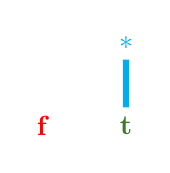
\begin{tikzpicture}[scale=0.35]
				 			\node (A) at (0,0) {\textcolor{red}{\textbf{f}}};
				 			\node (B) at (3,0) {\textcolor{OliveGreen}{\textbf{t}}};
				 			\node (C) at (3,3) {\textcolor{cyan}{$*$}};
				 			\draw[cyan, line width=.03in] (B) -- (C);
				 		\end{tikzpicture} \\
			 		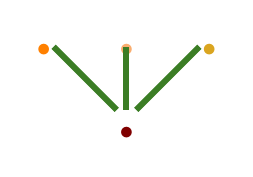
\begin{tikzpicture}[scale=0.35]
				 			\node (A) at (0,0) {\textcolor{OliveGreen}{$\bigcdot$}};
				 			\node (a) at (0,-0.5) {\textcolor{Maroon}{$\bullet$}};
				 			\node (B) at (-3,3) {\textcolor{OliveGreen}{$\bigcdot$}};
				 			\node (b) at (-3,2.5) {\textcolor{orange}{$\bullet$}};
				 			\node (C) at (0,3) {\textcolor{OliveGreen}{$\bigcdot$}};
				 			\node (c) at (0,2.5) {\textcolor{Apricot}{$\bullet$}};
				 			\node (D) at (3,3) {\textcolor{OliveGreen}{$\bigcdot$}};
				 			\node (d) at (3,2.5) {\textcolor{Goldenrod}{$\bullet$}};
				 			\draw[OliveGreen, line width=.03in] (A) -- (B);
				 			\draw[OliveGreen, line width=.03in] (A) -- (C);
				 			\draw[OliveGreen, line width=.03in] (A) -- (D);
				 		\end{tikzpicture} & 	
\begin{tikzpicture}[scale=0.35]
				 		\node (E) at (-6,0) {\textcolor{red}{$\bigcdot$}};			
				 		
				 		\node (A) at (0,0) {\textcolor{OliveGreen}{$\bigcdot$}};
				 		\node (B) at (-3,3) {\textcolor{OliveGreen}{$\bigcdot$}};
				 		\node (C) at (0,3) {\textcolor{OliveGreen}{$\bigcdot$}};
				 		\node (D) at (3,3) {\textcolor{cyan}{$\bigcdot$}};
				 		\draw[OliveGreen, line width=.03in] (A) -- (B);
				 		\draw[OliveGreen, line width=.03in] (A) -- (C);
				 		\draw[cyan, line width=.03in] (A) -- (D);
				 		
				 		\node (A') at (9,0) {\textcolor{OliveGreen}{$\bigcdot$}};
				 		\node (a) at (9,-1) {\textcolor{Maroon}{$\bullet$}};
				 		\node (a') at (8.5,-0.5) {\textcolor{orange}{$\bullet$}};
				 		\node (a'') at (9,-0.5) {\textcolor{Apricot}{$\bullet$}};
				 		\node (a''') at (9.5,-0.5) {\textcolor{Goldenrod}{$\bullet$}};
				 		\node (B') at (6,3) {\textcolor{OliveGreen}{$\bigcdot$}};
				 		\node (C') at (9,3) {\textcolor{OliveGreen}{$\bigcdot$}};
				 		\node (D') at (12,3) {\textcolor{cyan}{$\bigcdot$}};
				 		\draw[OliveGreen, line width=.03in] (A') -- (B');
				 		\draw[OliveGreen, line width=.03in] (A') -- (C');
				 		\draw[cyan, line width=.03in] (A') -- (D');
				 		\end{tikzpicture}  \\
			 		& 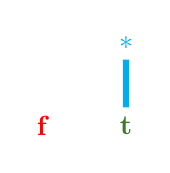
\begin{tikzpicture}[scale=0.35]
				 			\node (A) at (0,0) {\textcolor{red}{\textbf{f}}};
				 			\node (B) at (3,0) {\textcolor{OliveGreen}{\textbf{t}}};
				 			\node (C) at (3,3) {\textcolor{cyan}{$*$}};
				 			\draw[cyan, line width=.03in] (B) -- (C);
				 		\end{tikzpicture}
			 		\arrow["{pr^1_3 \times pr^3_3}"', from=1-1, to=1-2]
			 		\arrow["{\llbracket \textbf{P}_*(x_2) \rrbracket}"', from=1-2, to=1-3]
			 		\arrow["{| \textbf{P}_*(x_2) |_1^2}", from=2-1, to=2-2]
			 		\arrow["{\exists_{\textbf{1}_\bot}}", from=2-2, to=3-2]
			 		\arrow["{\llbracket \exists x_2.\textbf{P}_*(x_2) \rrbracket}"', from=2-1, to=3-2]
			 	\end{tikzcd}
		 	\caption{Again we find: $\llbracket \exists x_2. \textbf{P}_*(x_2) \rrbracket = \llbracket \textbf{P}_t(x_2) \rrbracket$.}
		 \end{figure}	
		 ...\newline
		 \newline
		 \newline
		 \newline
		 \newline
		 \newline
		 \newline
		 \newline
		 \newline
		 \newline
		 \newline
		 \newline
		 \newline
		 \newline
		 \newline
		 ...
		 \newline
		 \newline
		 \newline
		 \newline
		 \newline
		 \newline
		 \newline
		 \newline
		 \newline
		 \newline
		 \newline
		 \newline
		 \newline
		 \newline
		 \newline
		 \newline
		 ...
		 \newline
		 \newline
		 \newline
		 \newline
		 \newline
		 \newline
		 \newline
		 \newline
		 \newline
		 \newline
		 \newline
		 \newline
		 \newline
		 \newline
		 		 ...
		 \newline
		 \newline
		 \newline
		 \newline
		 \newline
		 \newline
		 \newline
		 \newline
		 \newline
		 \newline
		 \newline
		 \newline
		 \newline
		 \newline
		 		 ...
		 \newline
		 \newline
		 \newline
		 \newline
		 \newline
		 \newline
		 \newline
		 \newline
		 \newline
		 \newline
		 \newline
		 \newline
		 \newline
		 \newline
		 		 ...
		 \newline
		 \newline
		 \newline
		 \newline
		 \newline
		 \newline
		 \newline
		 \newline
		 \newline
		 \newline
		 \newline
		 \newline
		 \newline
		 \newline
	
		 \newpage
		 \subsection{From Predicates to Relations.}
		 
		 We introduce a \emph{relation} \textbf{R} of arity 2  realized by $\textfrak{r}$.
		 
		 \begin{figure}[h]
		 	\centering
		 	\begin{tikzcd}
			 			\begin{tikzpicture}[scale=0.35]
				 			\node (A) at (0,0) {\textcolor{OliveGreen}{$\bigcdot$}};
				 			\node (B) at (-3,3) {\textcolor{cyan}{$\bigcdot$}};
				 			\node (C) at (0,3) {\textcolor{OliveGreen}{$\bigcdot$}};
				 			\node (D) at (3,3) {\textcolor{cyan}{$\bigcdot$}};
				 			\draw[cyan, line width=.03in] (A) -- (B);
				 			\draw[OliveGreen, line width=.03in] (A) -- (C);
				 			\draw[cyan, line width=.03in] (A) -- (D);
				 		\end{tikzpicture} && \begin{tikzpicture}[scale=0.35]
				 			\node (A) at (0,0) {\textcolor{red}{\textbf{f}}};
				 			\node (B) at (3,0) {\textcolor{OliveGreen}{\textbf{t}}};
				 			\node (C) at (3,3) {\textcolor{cyan}{$*$}};
				 			\draw[cyan, line width=.03in] (B) -- (C);
				 		\end{tikzpicture}
			 		\arrow["\textfrak{r}", from=1-1, to=1-3]
			 	\end{tikzcd}
		 	\caption{$\textfrak{r} : (\textbf{1}_\bot \times \textbf{1}_\bot) \rightarrow \Omega$:}
		 \end{figure}
		 
		 \begin{ex} (m=2)
		 	\begin{gather*}
			 		\textfrak{X}= \langle \textbf{1}_\bot, \textfrak{r}, \textfrak{f}_c \rangle. \\ \\
			 		\llbracket x_1 \rrbracket = {pr_1} : (\textbf{1}_\bot \times \textbf{1}_\bot) \rightarrow \textbf{1}_\bot. \\
			 		\llbracket x_2 \rrbracket = {pr_2} : (\textbf{1}_\bot \times \textbf{1}_\bot) \rightarrow \textbf{1}_\bot. \\
			 		\llbracket \textbf{c} \rrbracket = \textfrak{f}_c \circ \; !_{\textbf{1}_\bot \times \textbf{1}_\bot} : (\textbf{1}_\bot \times \textbf{1}_\bot) \rightarrow \textbf{1}_\bot.  \\
			 		\llbracket \textbf{R}(x_1,x_2) \rrbracket = \textfrak{r} \circ (\llbracket x_1 \rrbracket \times \llbracket x_2 \rrbracket) = \textfrak{r} \circ id_{\textbf{1}_\bot \times \textbf{1}_\bot} = \textfrak{r}. \\
			 		\llbracket \textbf{R}(x_1,x_1) \rrbracket = \textfrak{r} \circ (\llbracket x_1 \rrbracket \times \llbracket x_1 \rrbracket). \\
			 		\llbracket \textbf{R}(x_1,\textbf{c}) \rrbracket = \textfrak{r} \circ (\llbracket x_1 \rrbracket \times \llbracket \textbf{c} \rrbracket). \\
			 		...
			 	\end{gather*}
		 \end{ex}
		 
		 
		 
		 \begin{figure}[h]
		 	\begin{tikzcd}
			 			\begin{tikzpicture}[scale=0.35]
				 			\node (A) at (0,0) {\textcolor{OliveGreen}{$\bigcdot$}};
				 			\node (a) at (0,-0.5) {\textcolor{Maroon}{$\bullet$}};
				 			\node (B) at (-3,3) {\textcolor{OliveGreen}{$\bigcdot$}};
				 			\node (b) at (-3,2.5) {\textcolor{orange}{$\bullet$}};
				 			\node (C) at (0,3) {\textcolor{OliveGreen}{$\bigcdot$}};
				 			\node (c) at (0,2.5) {\textcolor{Apricot}{$\bullet$}};
				 			\node (D) at (3,3) {\textcolor{OliveGreen}{$\bigcdot$}};
				 			\node (d) at (3,2.5) {\textcolor{Goldenrod}{$\bullet$}};
				 			\draw[OliveGreen, line width=.03in] (A) -- (B);
				 			\draw[OliveGreen, line width=.03in] (A) -- (C);
				 			\draw[OliveGreen, line width=.03in] (A) -- (D);
				 		\end{tikzpicture} && 	\begin{tikzpicture}[scale=0.35]
				 		\node (A) at (0,0) {\textcolor{OliveGreen}{$\bigcdot$}};
				 		\node (a) at (-0.5,-0.5) {\textcolor{Maroon}{$\bullet$}};
				 		\node (a') at (0.5,-0.5) {\textcolor{Goldenrod}{$\bullet$}};
				 		\node (B) at (-3,3) {\textcolor{cyan}{$\bigcdot$}};
				 		\node (C) at (0,3) {\textcolor{OliveGreen}{$\bigcdot$}};
				 		\node (c') at (-0.5,2.5) {\textcolor{orange}{$\bullet$}};
				 		\node (c) at (0.5,2.5) {\textcolor{Apricot}{$\bullet$}};	
				 		\node (D) at (3,3) {\textcolor{cyan}{$\bigcdot$}};
				 		\draw[cyan, line width=.03in] (A) -- (B);
				 		\draw[OliveGreen, line width=.03in] (A) -- (C);
				 		\draw[cyan, line width=.03in] (A) -- (D);
				 		\end{tikzpicture} \\
			 		\\
			 		&& \begin{tikzpicture}[scale=0.35]
				 			\node (A) at (0,0) {\textcolor{red}{\textbf{f}}};
				 			\node (B) at (3,0) {\textcolor{OliveGreen}{\textbf{t}}};
				 			\node (C) at (3,3) {\textcolor{cyan}{$*$}};
				 			\draw[cyan, line width=.03in] (B) -- (C);
				 		\end{tikzpicture}
			 		\arrow["{\llbracket x_1 \rrbracket \times \llbracket x_1 \rrbracket}", from=1-1, to=1-3]
			 		\arrow["r", from=1-3, to=3-3]
			 		\arrow["{\llbracket \textbf{R}(x_1,x_1) \rrbracket}"', from=1-1, to=3-3]
			 	\end{tikzcd}
		 	\caption{$	\llbracket \textbf{R}(x_1,x_1) \rrbracket = true_{\textbf{1}_\bot \times \textbf{1}_\bot}$.}
		 \end{figure}
		 
		  
		 \begin{figure}[h]
		 	\begin{tikzcd}
			 		\begin{tikzpicture}[scale=0.35]
				 			\node (A) at (0,0) {\textcolor{OliveGreen}{$\bigcdot$}};
				 			\node (a) at (0,-0.5) {\textcolor{Maroon}{$\bullet$}};
				 			\node (B) at (-3,3) {\textcolor{OliveGreen}{$\bigcdot$}};
				 			\node (b) at (-3,2.5) {\textcolor{orange}{$\bullet$}};
				 			\node (C) at (0,3) {\textcolor{cyan}{$\bigcdot$}};
				 			\node (c) at (0,2.5) {\textcolor{Apricot}{$\bullet$}};
				 			\node (D) at (3,3) {\textcolor{cyan}{$\bigcdot$}};
				 			\node (d) at (3,2.5) {\textcolor{Goldenrod}{$\bullet$}};
				 			\draw[OliveGreen, line width=.03in] (A) -- (B);
				 			\draw[cyan, line width=.03in] (A) -- (C);
				 			\draw[cyan, line width=.03in] (A) -- (D);
				 		\end{tikzpicture} && 	\begin{tikzpicture}[scale=0.35]
				 			\node (A) at (0,0) {\textcolor{OliveGreen}{$\bigcdot$}};
				 			\node (a) at (-0.5,-0.5) {\textcolor{Maroon}{$\bullet$}};
				 			\node (a') at (0.5,-0.5) {\textcolor{orange}{$\bullet$}};
				 			\node (B) at (-3,3) {\textcolor{cyan}{$\bigcdot$}};
				 			\node (C) at (0,3) {\textcolor{OliveGreen}{$\bigcdot$}};
				 			\node (D) at (3,3) {\textcolor{cyan}{$\bigcdot$}};
				 			\node (d) at (2.5,2.5) {\textcolor{Apricot}{$\bullet$}};
				 			\node (d') at (3.5,2.5) {\textcolor{Goldenrod}{$\bullet$}};
				 			\draw[cyan, line width=.03in] (A) -- (B);
				 			\draw[OliveGreen, line width=.03in] (A) -- (C);
				 			\draw[cyan, line width=.03in] (A) -- (D);
				 		\end{tikzpicture} \\
			 		\\
			 		&& \begin{tikzpicture}[scale=0.35]
				 			\node (A) at (0,0) {\textcolor{red}{\textbf{f}}};
				 			\node (B) at (3,0) {\textcolor{OliveGreen}{\textbf{t}}};
				 			\node (C) at (3,3) {\textcolor{cyan}{$*$}};
				 			\draw[cyan, line width=.03in] (B) -- (C);
				 		\end{tikzpicture}
			 		\arrow["{\llbracket \textbf{c} \rrbracket \times \llbracket x_2 \rrbracket}", from=1-1, to=1-3]
			 		\arrow["r", from=1-3, to=3-3]
			 		\arrow["{\llbracket \textbf{R}(\textbf{c},x_2) \rrbracket}"', from=1-1, to=3-3]
			 	\end{tikzcd}
		 	\caption{$	\llbracket \textbf{R}(\textbf{c},x_2) \rrbracket$.}
		 \end{figure}
